\documentclass{nitroma-article}
\usepackage[british]{babel}

% page layout
\usepackage{pdflscape}  % landscape pages
\usepackage{afterpage}  % full-page figures at the next opportunity
\usepackage{pdfpages}   % include other PDF docs

% typography
\usepackage{csquotes}   % clever quote marks
    \MakeOuterQuote{"}
\usepackage[detect-all]{siunitx} % numbers and units
    \DeclareSIUnit\year{yr}
    \DeclareSIUnit\USD{\$}
    \DeclareSIUnit\GBP{£}
    \DeclareSIUnit\EUR{€}
    \DeclareSIUnit\JPY{JP¥}
    \DeclareSIUnit\CNY{CN¥}
    \DeclareSIUnit\atm{atm}
    \DeclareSIQualifier\ww{w/w}
    \sisetup{text-celsius = °C}
\usepackage{enumitem}   % control list spacing
    \setlist{noitemsep}
% \usepackage{epigraph}

% formulae
\usepackage{amsmath}
\usepackage{chemmacros} % Swiss-army knife for chemistry

%comment out large sections
\usepackage{comment}

% graphics
\usepackage{graphicx}
\usepackage[font={small,singlespacing},labelfont={bf},skip=2pt]{caption}
\usepackage{subcaption}
\usepackage{wrapfig}
\usepackage{float}

% tables
\usepackage{tabularx}
    \newcolumntype{Y}{>{\centering\arraybackslash}X}
\usepackage{booktabs}
\usepackage{multirow}
\usepackage{multicol}
\usepackage{longtable}
\usepackage{colortbl}
\newcommand{\tabsup}[1]{\textsuperscript{\textit{#1}}}
\usepackage{adjustbox}

\newcommand{\splitcell}[2][t]{% https://tex.stackexchange.com/a/19678/135479
    \begin{tabular}[#1]{@{}c@{}}#2\end{tabular}}
\newcommand{\rtext}[2][90]{\rotatebox[origin=r]{#1}{#2}}
\newcommand{\rcell}[2][2cm]{\rtext{\parbox{#1}{\raggedleft #2}}} % ideally should use origin=rt https://tex.stackexchange.com/a/367139/135479 but that goes weird

\newcommand{\gLo}{\cellcolor{green}L}
\newcommand{\yMe}{\cellcolor{yellow}M}
\newcommand{\rHi}{\cellcolor{red}H}

% referencing
\usepackage[hidelinks]{hyperref} % clickable links
    \newcommand{\email}[1]{\href{mailto:#1}{\texttt{#1}}}
\usepackage[capitalise,noabbrev]{cleveref}   % clever cross-referencing
% \usepackage[titletoc]{appendix}
\usepackage[style=chem-angew,maxnames=3]{biblatex} % references
    \addbibresource{zotero.bib}
    \renewcommand*{\bibfont}{\scriptsize}
    \AtBeginBibliography{
        \setlength{\itemsep}{0em}
        \setlength{\parskip}{0em}
    }
\usepackage{nomencl}
    \makenomenclature
\usepackage{etoolbox}
    \renewcommand\nomgroup[1]{%
        \item[\bfseries
        \ifstrequal{#1}{A}{Acronyms}{%
        \ifstrequal{#1}{G}{General}{%
        \ifstrequal{#1}{X}{Superscripts}{%
        \ifstrequal{#1}{Z}{Subscripts}{%
        }}}}% same number of closing brackets as lines above
    ]\vspace{\parsep}}
    \setlength{\nomitemsep}{0pt}
    \renewcommand{\nompreamble}{\small}

\subtitle{Interim Design Report}
\title{Continuous Nitration of Substituted Aromatics}
\author{Team 8: Marie~Jones, Mathusan~Kandiah, Zong~Lee, Yuxin~Liu, Mustafa~Nasar, Helen~Ogbobi, Wei~Ooi, Andreas~Richardson, Stephen~Tan, Sathurthini~Thurairatnam, Mingchuan~Zheng}
\date{8 February 2021}

\begin{document}

\maketitle

% !TeX root = ../main.tex
\section*{Executive Summary}
\label{sec:exec-summary}

Substituted aromatic amines are essential intermediates involved in the synthesis of many pharmaceutical compounds, agrochemicals, and dyes \cite{vogt_amines_2000}. The amino group, which cannot be directly introduced via electrophilic aromatic substitution, is instead added via nitration and subsequent reduction. Following multiple deadly industrial accidents in chemical plants performing batch nitration, Chinese authorities are actively attempting to strengthen the control and management of nitration manufacturing \cite{el_diario_china_2019}.

In this context, Nitroma seizes the opportunity; developing an inherently safe, multi-purpose, continuous liquid-phase nitration process to produce o-toluidine, 4-aminobenzaldehyde and 4-aminobenzoic acid. This report details the preliminary design for Nitroma’s demonstration plant, to be located in the Nanjing Chemical Industry Park (China). Synthesis pathways for nitration, oxidation and hydrogenation reactions were selected and modelled in innovative packed-bed microreactors or trickle-bed reactors. Novel downstream processing units, including continuous falling-film melt crystallisers, enable Nitroma to reach the target product purity. Finally, a techno-economic feasibility study was conducted, taking into account health, safety and environmental considerations.

%% !TeX root = ../main.tex
\section{Introduction}
\label{sec:introduction}

% !TeX root = ../main.tex
\section{Process Synthesis }
\label{sec:synthesis}
\subsection{Decision analysis}
%explain TOPSIS and AHP
\noindent To make systematic and informed decisions for key aspects of the project, multi-criteria decision making (MCDM) methods were employed. Firstly, pairwise comparison of the criteria was performed with the Analytical Hierarchy Process (AHP) to produce criteria weightings which were fed into the Technique for Order of Preference by Similarity to Ideal Solution (TOPSIS) analysis. Processing of all relevant information through AHP and TOPSIS analysis yielded quantitative rankings for process alternatives, which were initially short-listed with qualitative arguments. Greater importance was given to safety and environmental concerns, technical performance and economic potential.


\subsection{Product selection}
\noindent To deliver a multi-purpose plant, Nitroma selected toluene as feedstock due to the industrial importance of its nitration products and their amino derivatives. All three isomeric nitrotoluenes can indeed easily be oxidised and reduced to substituted aromatic amides of significant importance for the pharmaceutical, agrochemical and textile industries \cite{dugal_nitrobenzene_2005}. Six chemicals were initially selected due to their applications in drugs, fertilizers or dyes \cite{bowers_toluidines_2000,bruhne_benzaldehyde_2011,maki_benzoic_2000}. To determine the three most advantageous products to produce, AHP/TOPSIS analysis was conducted, giving significant importance to the safety of the compounds and their economic potential. Safety was assessed using the NFPA Hazard Classification for health, flammability and instability, where the smallest value is preferable. The economic potential of each chemical was determined using the average price, the average market share of producers which is an indicator of the market share Nitroma can plan to capture, the golbal demand and the expected market growth (CAGR). \Cref{tab:product} summarises the results and the complete methodology can be found in \Cref{app:matrix}.   

\begin{comment}
\noindent To deliver a multi-purpose plant, Nitroma selected toluene as feedstock due to the industrial importance of its nitration products and their amino derivatives. All three isomeric nitrotoluenes can indeed easily be oxidised and reduced to substituted aromatic amides of significant importance for the pharmaceutical, agrochemical and textile industries \cite{dugal_nitrobenzene_2005}. Six chemicals were initially selected due to their applications in drugs, fertilizers or dyes: 2-aminobenzaldehyde (precursor of quinoline derivatives for polymer, agrochemical, dye, antiviral and anti-malaria drug manufacturing), 4-aminobenzaldehyde (intermediate to pharmaceuticals and vanilin), 4-aminobenzoic acid (production of folic acid/vitamin B9), \ortho-toluidine (intermediate in the manufacture of herbicides), \meta-toluidine (manufacture of  photographic color developer) and \para-toluidine (for dye production) \cite{bowers_toluidines_2000,bruhne_benzaldehyde_2011,maki_benzoic_2000}. To determine the three most advantageous products to produce, AHP/TOPSIS analysis was conducted, giving significant importance to the safety of the compounds and their economic potential. Safety was assessed using the NFPA Hazard Classification for health, flammability and instability, where the smallest value is preferable. The economic potential of each chemical was determined using the average price, the average market share of producers which is an indicator of the market share Nitroma can plan to capture, the golbal demand and the expected market growth (CAGR). \Cref{tab:product} summarises the results and the complete methodology can be found in \Cref{app:matrix}.   
\end{comment}


\begin{table}[h]
\centering
    \caption{AHP/TOPSIS results for product selection}
    \label{tab:product}\footnotesize
\begin{tabularx}{\linewidth}{l|S[table-format=4.2]S[table-format=1.1]XS[table-format=7.0,round-mode=figures,round-precision=2]|XX|lll|S[table-format=1.3]S[table-format=1.3]c}
\toprule
                                          & \multicolumn{4}{c}{Economic potential   (29\%)}                                & \multicolumn{2}{|>{\hsize=\dimexpr2\hsize+2\tabcolsep}X}{Process   complexity (14\%)} & \multicolumn{3}{|c|}{EHS (57\%)}     &                       &                          &                           \\ \cmidrule{2-10}
                                          & {\splitcell{Price\\(\si{\USD\per\kg})}} & {\splitcell{CAGR\\(\%)}} & \rcell{Average market share of producer (\%)} & {\splitcell{Demand\\(\si{\tonne\per\year})}} & \rcell{Number of reactions} & \rcell{Max selectivity to toluene (\%)} & \rotatebox[origin=r]{90}{Health} & \rotatebox[origin=r]{90}{Flammability} & \rotatebox[origin=r]{90}{Instability} & AHP & TOPSIS & Rank \\ \midrule
2-aminobenzaldehyde & 1711          & 5.6 & 0.77                           & 1344                 & 2                & 53                       & 2      & 1            & 1           & 0.124                 & 0.273                    & 6                         \\ 
4-aminobenzaldehyde & 19            & 7.1 & 1.75                           & 336842               & 2                 & 44                       & 2      & 1            & 0           & 0.188                 & 0.563                    & \cellcolor{green}2 \\ 
o-toluidine         & 5.8           & 7.8 & 0.88                           & 1327586              & 1                   & 53                       & 3      & 2            & 0           & 0.210                 & 0.611                    & \cellcolor{green}1 \\ 
p-toluidine         & 9             & 6.3 & 0.50                           & 722222               & 1                   & 44                       & 3      & 2            & 0           & 0.150                 & 0.333                    & 5                         \\ 
m-toluidine         & 8.9           & 8.2 & 0.57                           & 1067416              & 1                   & 3                       & 4      & 2            & 0           & 0.161                 & 0.458                    & 4                         \\ 
4-aminobenzoic acid & 26.29         & 5.8 & 3.70                           & 311906               & 2                 & 44                       & 2      & 1            & 1           & 0.168                 & 0.478                    & \cellcolor{green}3 \\ \bottomrule
\end{tabularx}
\end{table}

Due to their high economic potential and reduced health and fire hazards, 4-aminobenzaldehyde, o-toluidine and 4-aminobenzoic acid were found to be the most valuable compounds to be produced in Nitroma's multi-purpose plant.  A visual summary of the selected compounds and their associated synthesis pathways can be found in \Cref{app:kinetics}.


\subsection{Nitration method}
\subsubsection{Choice of nitrating agent}
\noindent Nitric acid, introduced as an aqueous solution, has been selected as the source of nitrogen for the nitration of toluene for its safe and environmentally friendly nature relative to alternatives such as acetone cyanohydrin and dinitrogen tetroxide, which are highly toxic \cite{miller_kinetics_1964,dagade_nitration_2002, sreedhar_scientific_2013}. 



\begin{comment}
\noindent Nitric acid has been selected as the source of nitrogen for the nitration of toluene for its safe and environmentally friendly nature relative to other possible nitrating agents, high availability, and its various favourable properties \cite{miller_kinetics_1964, sreedhar_scientific_2013}. Although nitric acid is a highly acidic and volatile compound, compared to alternatives such as acetone cyanohydrin and dinitrogen tetroxide which are highly toxic, nitric acid is more appropriate for industrial-scale nitration of toluene \cite{dagade_nitration_2002, sreedhar_scientific_2013}. Nitric acid, introduced as an aqueous solution, is the most commonly used and well-studied nitrating agent for this process in industry. \cite{bowers_toluidines_2000} A big advantage of aqueous nitric acid is that it can act as a self-catalyst by self-donating protons. \cite{miller_kinetics_1964} A common alternative to nitric acid is acetyl nitrate which is formed by the reaction of nitric acid with acetic anhydride. \cite{vassena_selective_1999} This reaction yields formic acid as by-product, resulting in a lower atom economy; it also causes unnecessary difficulties in separations downstream by introducing three extra components: acetyl nitrate, acetic anhydride, and formic acid. The same argument can be employed for other alkyl nitrates such as butyl nitrate. To this end, nitric acid is deemed as the most suitable choice among all candidates.
\end{comment}

\subsubsection{Choice of catalyst}
Nitration in industry is mainly carried out by a mixed-acid process []. In addition to favouring less economically desirable \textit{ortho} isomers, product separation from the acid and acid regeneration are expensive and energy intensive \cite{sreedhar_scientific_2013}. These drawbacks can be overcome by using solid acid catalysts which offer an environmentally friendly and economic alternative to sulfuric acid \cite{vassena_selective_1999}. Based on those arguments, Nitroma will develop a safer and low environmental impact process employing zeolite catalysts for toluene nitration. More specifically, the relative benefits and disadvantages of 3 different zeolites were evaluated with the AHP and TOPSIS decision analysis methods. The economic potential, performance and safety of zeolites H-ZSM-5, H-Y and H-Mordenite were assessed and compared to the case with no catalyst \cite{jeeru_kinetics_2018}. H-Mordenite was found optimum for the catalytic nitration of toluene by both AHP and TOPSIS analysis (see \Cref{tab:nitration} in \Cref{app:matrix}). The kinetic model for the reaction was then developed and is presented in \Cref{app:kinetics}.

\begin{comment}
Nitration in industry is mainly carried out by a mixed-acid process, whereby sulfuric acid donates a proton to nitric acid, yielding a nitronium ion which will then react with toluene []. In addition to favouring less economically desirable \textit{ortho} isomers, product separation from the acid and acid regeneration are expensive and energy intensive \cite{sreedhar_scientific_2013}. These drawbacks can be overcome by using solid acid catalysts which offer an environmentally friendly and economic alternative to sulfuric acid \cite{vassena_selective_1999}. Based on those arguments, Nitroma will develop a safer and low environmental impact process employing zeolite catalysts for toluene nitration. More specifically, the relative benefits and disadvantages of 3 different zeolites were evaluated with the AHP and TOPSIS decision analysis methods to select the optimum catalyst. The economic potential, performance and safety of zeolites H-ZSM-5, H-Y and H-Mordenite were assessed and compared to the case with no catalyst \cite{jeeru_kinetics_2018}. The economic potential was measured with the cost of the catalyst and the percentage of undesirable by-product formed. Conversion and the NFPA score are the KPIs for performance and safety respectively. H-Mordenite was found optimum for the catalytic nitration of toluene by both AHP and TOPSIS analysis (see \Cref{app:matrix}). The kinetic model for the reaction was then developed and is presented in \Cref{app:kinetics}.
\end{comment}

%assumptions
%catalyst selection process --> criteria + AHP/TOPSIS results


\subsection{Nitrotoluene Oxidation and hydrogenation pathways}
\subsubsection{\ortho-toluidine production}
\noindent The \textit{ortho} isomer of nitrotoluene is reduced to o-toluidine using  2\% w/w palladium-on-carbon (Pd/C) catalyst in the liquid-phase \cite{rajadhyaksha_solvent_1986}. This reaction is carried out in a solvent to dissolve solid reactants and products, absorb the heat of exothermic reaction and protect the catalyst surface from impurities []. Five different solvents were compared using AHP/TOPSIS analysis to determine the optimum solvent based on economic potential, performance, safety and environmental considerations. The performance of a solvent was measures through the activation energy of the reaction, the reaction rate at 333K and the solubility of \ch{H2} in the solvent \cite{rajadhyaksha_solvent_1986}. Nitroma values the importance of using green solvents in its process and evaluated the sustainability of the different solvents using scores developed by GSK to assess the environmental impacts to produce the solvent, waste treatment and the fate and effects of the chemicals on the environment \cite{henderson_expanding_2011}. The GSK scored for health and flammability were also used for safety. If a solvent could be sourced from renewable feed stocks, it was viewed positively \cite{byrne_tools_2016}. Both TOPSIS and AHP found that propanol was the most suitable green solvent for the reduction of 2-nitrotoluene (see \Cref{tab:solvent} in \Cref{app:matrix}). 

\begin{comment}
\noindent The \textit{ortho} isomer of nitrotoluene (53\%) is reduced to o-toluidine using  2\% w/w palladium-on-carbon (Pd/C) catalyst in the liquid-phase \cite{rajadhyaksha_solvent_1986}. This reaction is carried out in a solvent to dissolve solid reactants and products, absorb the heat of exothermic reaction and protect the catalyst surface from impurities. The chosen solvent can significantly affect the rate and selectivity of the hydrogenation []. Five different solvents, including methanol, propanol, butanol, cyclohexanol and hexane, were compared using AHP/TOPSIS analysis to determine the optimum solvent based on economic potential, performance, safety and environmental considerations. The performance of a solvent was measures through the activation energy of the reaction, the reaction rate at 333K and the solubility of \ch{H2} in the solvent \cite{rajadhyaksha_solvent_1986}. The financial KPI is solvent cost. Nitroma values this importance of using green solvents in its process and evaluated the sustainability of the different solvents using scores developed by GSK to assess the environmental impacts to produce the solvent, waste treatment and the fate and effects of the chemicals on the environment \cite{henderson_expanding_2011}. The GSK scored for health and flammability were also used. If a solvent could be sourced from renewable feed stocks, it was viewed positively \cite{byrne_tools_2016}. Both TOPSIS and AHP found that propanol was the most suitable green solvent for the reduction of 2-nitrotoluene. The table of scores is located in \Cref{app:matrix}.
\end{comment}


%In all the above runs, the rates of reaction remained constant in each experiment for a conversion of more than 90\%, indicating zero-order dependence on the concentration of the nitro compound. The results indicate a 0.3 order dependence on hydrogen pressure or first order for pressure >280 kPa

\subsubsection{4-nitrotoluene oxidation}

\subsubsection{4-aminobenzoic acid and 4-aminobenzaldehyde synthesis}



%assumptions
%catalyst/solvent/reductant/oxidant selection process --> criteria + AHP/TOPSIS results
%kinetics derivation


% !TeX root = ../main.tex
\section{Process description}
\label{sec:process}
\subsection{Nitration step}
%reactor design
%selection criteria
%innovation
In line with Nitroma's goal of transitioning from batch to continuous process, packed-bed microreactors were chosen for the nitration of toluene. Due to their high surface area to volume ratio, microreactors are superior in heat transfer as compared to conventional batch or semi-batch reactors []. This was an important criteria when choosing nitration reactors as nitration is a highly exothermic process with the hazard of thermal runaway if the temperature is not controlled. Additionally, microreactors offer the benefit

There has been an increasing interest in deploying microreactors on large scale nitration processes, but most industrial nitration reactors are still limited to batch and semi-batch processes. Therefore, Nitroma is poised to gain the first mover advantage by designing a safe and 
(Alternative continuous reactors were considered in Appendix [ ])
The catalysts in the microreactors were 
\subsection{Nitrotoluene isomers separation}



\subsection{o-toluidine production}
%trickle bed reactor
%Pd/c catalyst
For the o-toluidine hydrogenation, a cocurrent trickle bed reactor was selected
with both gas and liquid reactants flowing downwards. Trickle bed reactor was chosen due to the ease of operation at high pressure (13 atm) and the relative slow catalyst deactivation, which is imperative for an expensive catalyst usage of Pd. Moreover, the plug flow liquid flow in trickle bed reactor allows for a higher conversion than other reactors, matching  the 90\% conversion rate target of o-toluidine by Nitroma. 


%assumptions to be added in appendix
\subsection{4-nitrotoluene oxidation}

\subsection{4-nitrobenzoic acid and 4-nitrobenzaldehyde hydrogenation}


\subsection{Major equipment sizing}
%to be added in appendix?

\subsection{Process alternatives}
%to be added in appendix? --> just mention them here and refer to appendix but we need it here too


%nitration synthesis --> with mixed acid
%funky intensified reactors
%2nd best reactor type --> 
%direct or indirect 4-amino production --> one pot 
% !TeX root = ../main.tex
\section{Business assessment}
\label{sec:economics}
\subsection{Selection of location} 
AHP and TOPSIS methodologies were used to determine a suitable country for Nitroma’s chemical plant. The key factors taken into consideration are summarised in Table XX in Appdendix XX. China was identified as the optimal country for Nitroma's plant, owing to its strong local supply chain and low business operating costs. A sensitivity analysis was performed on the decision criteria, but none of the scenarios downgraded China. To identify an optimal city within China, the spread of toluene suppliers, access to distribution channels, local market demand and business policies across the provinces of China were studied. The Nanjing Jiangbei New Material Science Park located in Nanjing, Jiangsu was selected. China’s largest toluene manufactory, operated by Sinopec Yangzi Petrochemical, is situated within 10 km of Nitroma’s selected site in Jiangsu (XX). The Jiangsu province also hosts 20\% of China’s inland waterways and 4,710 km of highways, creating reliable access to the neighbouring Shanghai Port and markets in Shandong and Zhegiang (XX). Moreover, Jiangsu operates a favourable policy towards foreign-owned and private businesses (XX). 

\subsection{Business model} 
\subsubsection{Business plan}
Nitroma will operate as a contract manufacturing organisation (CMO), developing a continuous nitration process to produce 4-aminobenzaldehyde (≥ 98\%), 4-aminobenzoic acid (≥ 98\%) and o-toluidine (≥ 95\%). The target markets for these products are the local dye, pharmaceutical and agrochemical industries in China.
\subsubsection{Industry landscape}
The Chinese markets for Nitroma’s three products are highly fragmented, with the average market share for 4-aminobenzaldehyde, 4-aminobenzoic acid and o-toluidine summarised in Table XX. The industry structure can be defined as monopolistic competition where Nitroma reserves pricing power. In recent times, growing concerns around safety have led Chinese authorities to introduce upgraded safety legislation and operating requirements for chemical sites (XX). In 2019, Jiangsu shut down 9 chemical parks (equivalent to 244 chemical plants) due to safety risks (XX). Incumbents and newcomers in the Chinese chemicals market will have to adapt fast to survive the challenging phase of increased regulatory control. 
\subsubsection{Value proposition}
Nitroma seeks the reward of fulfilling unmet demand as many of its competitors are removed from the market. Nitroma’s inherently safe design means it is not threatened by closures, making it a more reliable supplier for buyers to enter long-term purchasing contracts with. The unique continuous nature of Nitroma’s nitration process also means improved product quality – an important characteristic for Nitroma’s pharmaceutical customer segment. Moreover, Nitroma’s built-in production flexibility gives buyers the option to renegotiate contracts as their needs evolve. Finally, Nitroma offers convenience to buyers due its diversity of aromatic amine products, making it an attractive “one-stop shop”.
\subsubsection{Economic model: cost leadership}
Nitroma is positioned to leverage recent tax subsidisation policies set by the Chinese Ministry of Commerce related to safe process designs [XX]. Nitroma aims to follow the example of its industry peers, such as Yangmei Chemical which received 62 subsidies worth USD 10.1 million for transitioning to energy-efficient equipment in 2020 [XX]. Moreover, employing a continuous process will allow Nitroma to cut operating costs by improving its hourly production rate and resource efficiency, whilst reducing operating expenditure. As a result, Nitroma can set a below-market price point for its product line and still generate a healthy profit margin. This competitive advantage will allow Nitroma to acquire market share from industry incumbents. 
\subsubsection{Mode of operation: WFOE}
Nitroma will establish itself as a wholly foreign-owned enterprise (WFOE) in China. Being a high-tech company with a physical footprint, operating as a WFOE will allow Nitroma to register a legal presence in China and so, own real estate and intellectual property under its own name. Another important aspect of operating as a WFOE is that Nitroma will have independent management of its processes, making it easier to negotiate contracts with buyers under its CMO-styled operations.

\subsection{Production capacity}
Nitroma’s annual production and market share targets are summarised in Table XX. These numbers are based on the local product demand and average market share of competitors, detailed in Table 1. The targets are set for the first 5 years of Nitroma’s operations, with the possibility of a future expansion under investigation. Nitroma is confident its business strategy, outlined in Section XX, will allow it to achieve these targets. 

\begin{table}[h]
\centering
\caption{Production capacity}
\label{tab:production-capacity}
\begin{tabular}{lcc} 
\toprule
Product & Annual production (t/yr) & Market share (\%) \\ \midrule
4-aminobenzaldehyde & 0-500 & 1.50 \\ 
4-aminobenzoic acid & 0-100 & 3.00 \\ 
o-toluidine & 0-650 & 0.10 \\ 
\bottomrule
\end{tabular}
\end{table}

\subsection{Market analysis}

\subsubsection{Feedstock Supply}
Toluene is used in construction, explosions and agrochemicals which drives the domestic demand for it in China \cite{reportbuyer_global_nodate} . The price of toluene is susceptible to fluctuating prices in crude oil which leads to fluctuating global supply and demand \cite{noauthor_toluene_nodate-1}. China had plant expansions in 2019 \cite{zhang_china_nodate} therefore domestic production of toluene is expected to increase and provide reliable supply \cite{noauthor_toluene_nodate}. Toluene will be sourced from Sinopec Yangzi Petrochemical in Jiangsu, China[].


\subsection{Economic analysis}
% !TeX root = ../main.tex
\section{Environmental, Health and Safety (EHS) Considerations}
\label{sec:ehs}

\nomenclature[A]{EHS}{Environmental, health and safety}

Nitroma demonstrates the prioritization of EHS considerations are by complying to all relevant safety and environmental regulations as listed in Appendix \ref{app:EHS}. 

\subsection{Health and Safety}
Inherent safety was a fundamental element of the design stage. The continuous nature of the process presents a safer alternative to batch operation, as it requires a smaller inventory and reduces threat of thermal runaway caused by hot-spot formation []. Furthermore, a continuous process will allow adaptable automatic control, eliminating the need for manual handling and thus reducing risks associated with human error \cite{mannan_lees_2012}. A key substitution was the choice of nitration catalyst, with H-mordenite favoured over concentrated sulphuric acid which is highly corrosive and reactive. Moderations were made in terms of plant layout, isolating the hazardous process units as much as reasonable, preventing sequential events should a fire or explosion occur. To simplify the overall design of the plant a minimal number of reaction and separation units were chosen, lowering the complexity of the plant whilst enabling specified process targets to be met. 

%Inherent safety was a fundamental element of the design stage. The hazardous inventory has been reduced by using toluene as the initial feedstock material for all final products. The continuous nature of the process presents a safer alternative to batch operation, as it requires a smaller inventory and reduces threat of thermal runaway due to hot-spot formation. Furthermore, a continuous process will allow adaptable automatic control, eliminating the need for manual handling and thus reduces risks associated with human error \cite{mannan_lees_2012}. A key substitution was the choice the nitration catalyst, with H-mordenite favoured over concentrated sulphuric acid which is highly corrosive and reactive. Moderations were made in terms of plant layout, isolating the hazardous process units as much as possible, preventing sequential events should a fire or explosion occur. To simplify the overall design of the plant a minimal number of reaction and separation units were chosen, lowering the complexity of the plant whilst enabling specified process targets to be met. 

The specific hazards of each chemical component have been considered, with the NFPA 704 values, flash point value, auto-ignition temperature, vapour pressure and Globally Harmonized System Hazards found in\Cref{tab:chemID}. All substances have a relatively low reactivity rating. There are two oxidisers present (nitric acid and oxygen) and the most flammable substance identified was hydrogen gas.  

Fires, explosions and the release of toxic substances are the typical consequences of the major process hazards which can occur in a chemical plant \cite{mannan_lees_2012}. For each of the main hazards identified that may result in the occurrence of these events, the risk was estimated in a qualitative approach using the severity-likelihood risk matrix, found in \Cref{tab:risk-matrix}. For a quantitative hazard assessment, Dow's Fire and Explosion Index was utilised to identify which specific process units are most liable to  a fire, blast or explosion occurring, sizing the amount of damage it would inflect should the incident occur (\Cref{app:EHS}). This essential identification and analysis permits the selection of appropriate actions and controls to mitigate potential process hazards. This includes integrating appropriate temperature and pressure monitors into reactors, the fitting of cooling jackets and firewalls, and the selection of material best suited to prevent loss of containment.


\subsection{Environmental Impact}

The modular nature of the process plant indicates waste streams will be identified at various units across the plant. Following guidance from the Green Engineering Principles and the waste hierarchy system, efforts have been made to prevent waste where possible. The traditional method of nitration involves the use of sulphuric acid, however disposal of the ‘spent’ acid is environmentally unfriendly and costly and thus a recyclable zeolite catalyst was chosen \cite{smith_superior_1996}.  Formic acid was chosen as a reducing agent for the hydrogenation reactions over ammonium formate to prevent the emission of  ammonia. Furthermore, energy recovery is being considered from the waste stream of nitration by utilising the energy for heat exchange from the nitric acid and water mixture. 
%The toluene for the nitration solvent will be re-used through a recovery system.

Despite efforts made, the presence of waste is inevitable and so a list of the best available techniques was devised in the Appendix (xx), the treatment ensuring compliance with regarding threshold limits. The Environment Agency states that the maximum threshold limits for the biological oxygen demand and chemical oxygen demand are \SIlist{50;250}{\mg\of{\ch{O2}}\per\l} respectively, whilst the maximum concentration limit of total nitrogen is \SI{15}{\mg\of{\ch{N}}\per\l} \cite{govuk_waste_nodate}. 
\section{Conclusions and Outlook}
\label{sec:conclu}
Nitroma is designed a multi-purpose plant for the nitration of toluene and subsequent oxidation and hydrogenation of nitrotoluene isomers to valuable substituted amines. The control of nitrotoluene oxidation enables to switch production line and offers great production flexibility. Most importantly, Nitroma developed a continuous liquid-phase nitration process, replacing hazardous sulfuric acid with zeolite catalyst. Continuous operation of packed-bed microreactor diminishes the risks of hot-spot formation and thermal runaways, typical of traditional batch processes. Nitroma aims at taking advantage of the favourable economic and political situation in China to implement its innovative process, while ensuring complete compliance to the new health, safety and environmental regulations in place. Further work includes mechanical design of the reactor and separation units as well as the establishment of a robust control system for the process. 

\clearpage
\twocolumn
\printbibliography
\clearpage
\printnomenclature
\onecolumn

%you did the one column or did i break something?

\clearpage
\appendix
% number figures and tables in the appendices as A.1 etc
\numberwithin{figure}{section}
\numberwithin{table}{section}
% \begin{appendices}
% !TeX root = ../main.tex
\section{Process Flow Diagram}
\label{app:PFD}

Following this page is attached the preliminary process flow diagram (PFD) for Nitroma's proposed process.

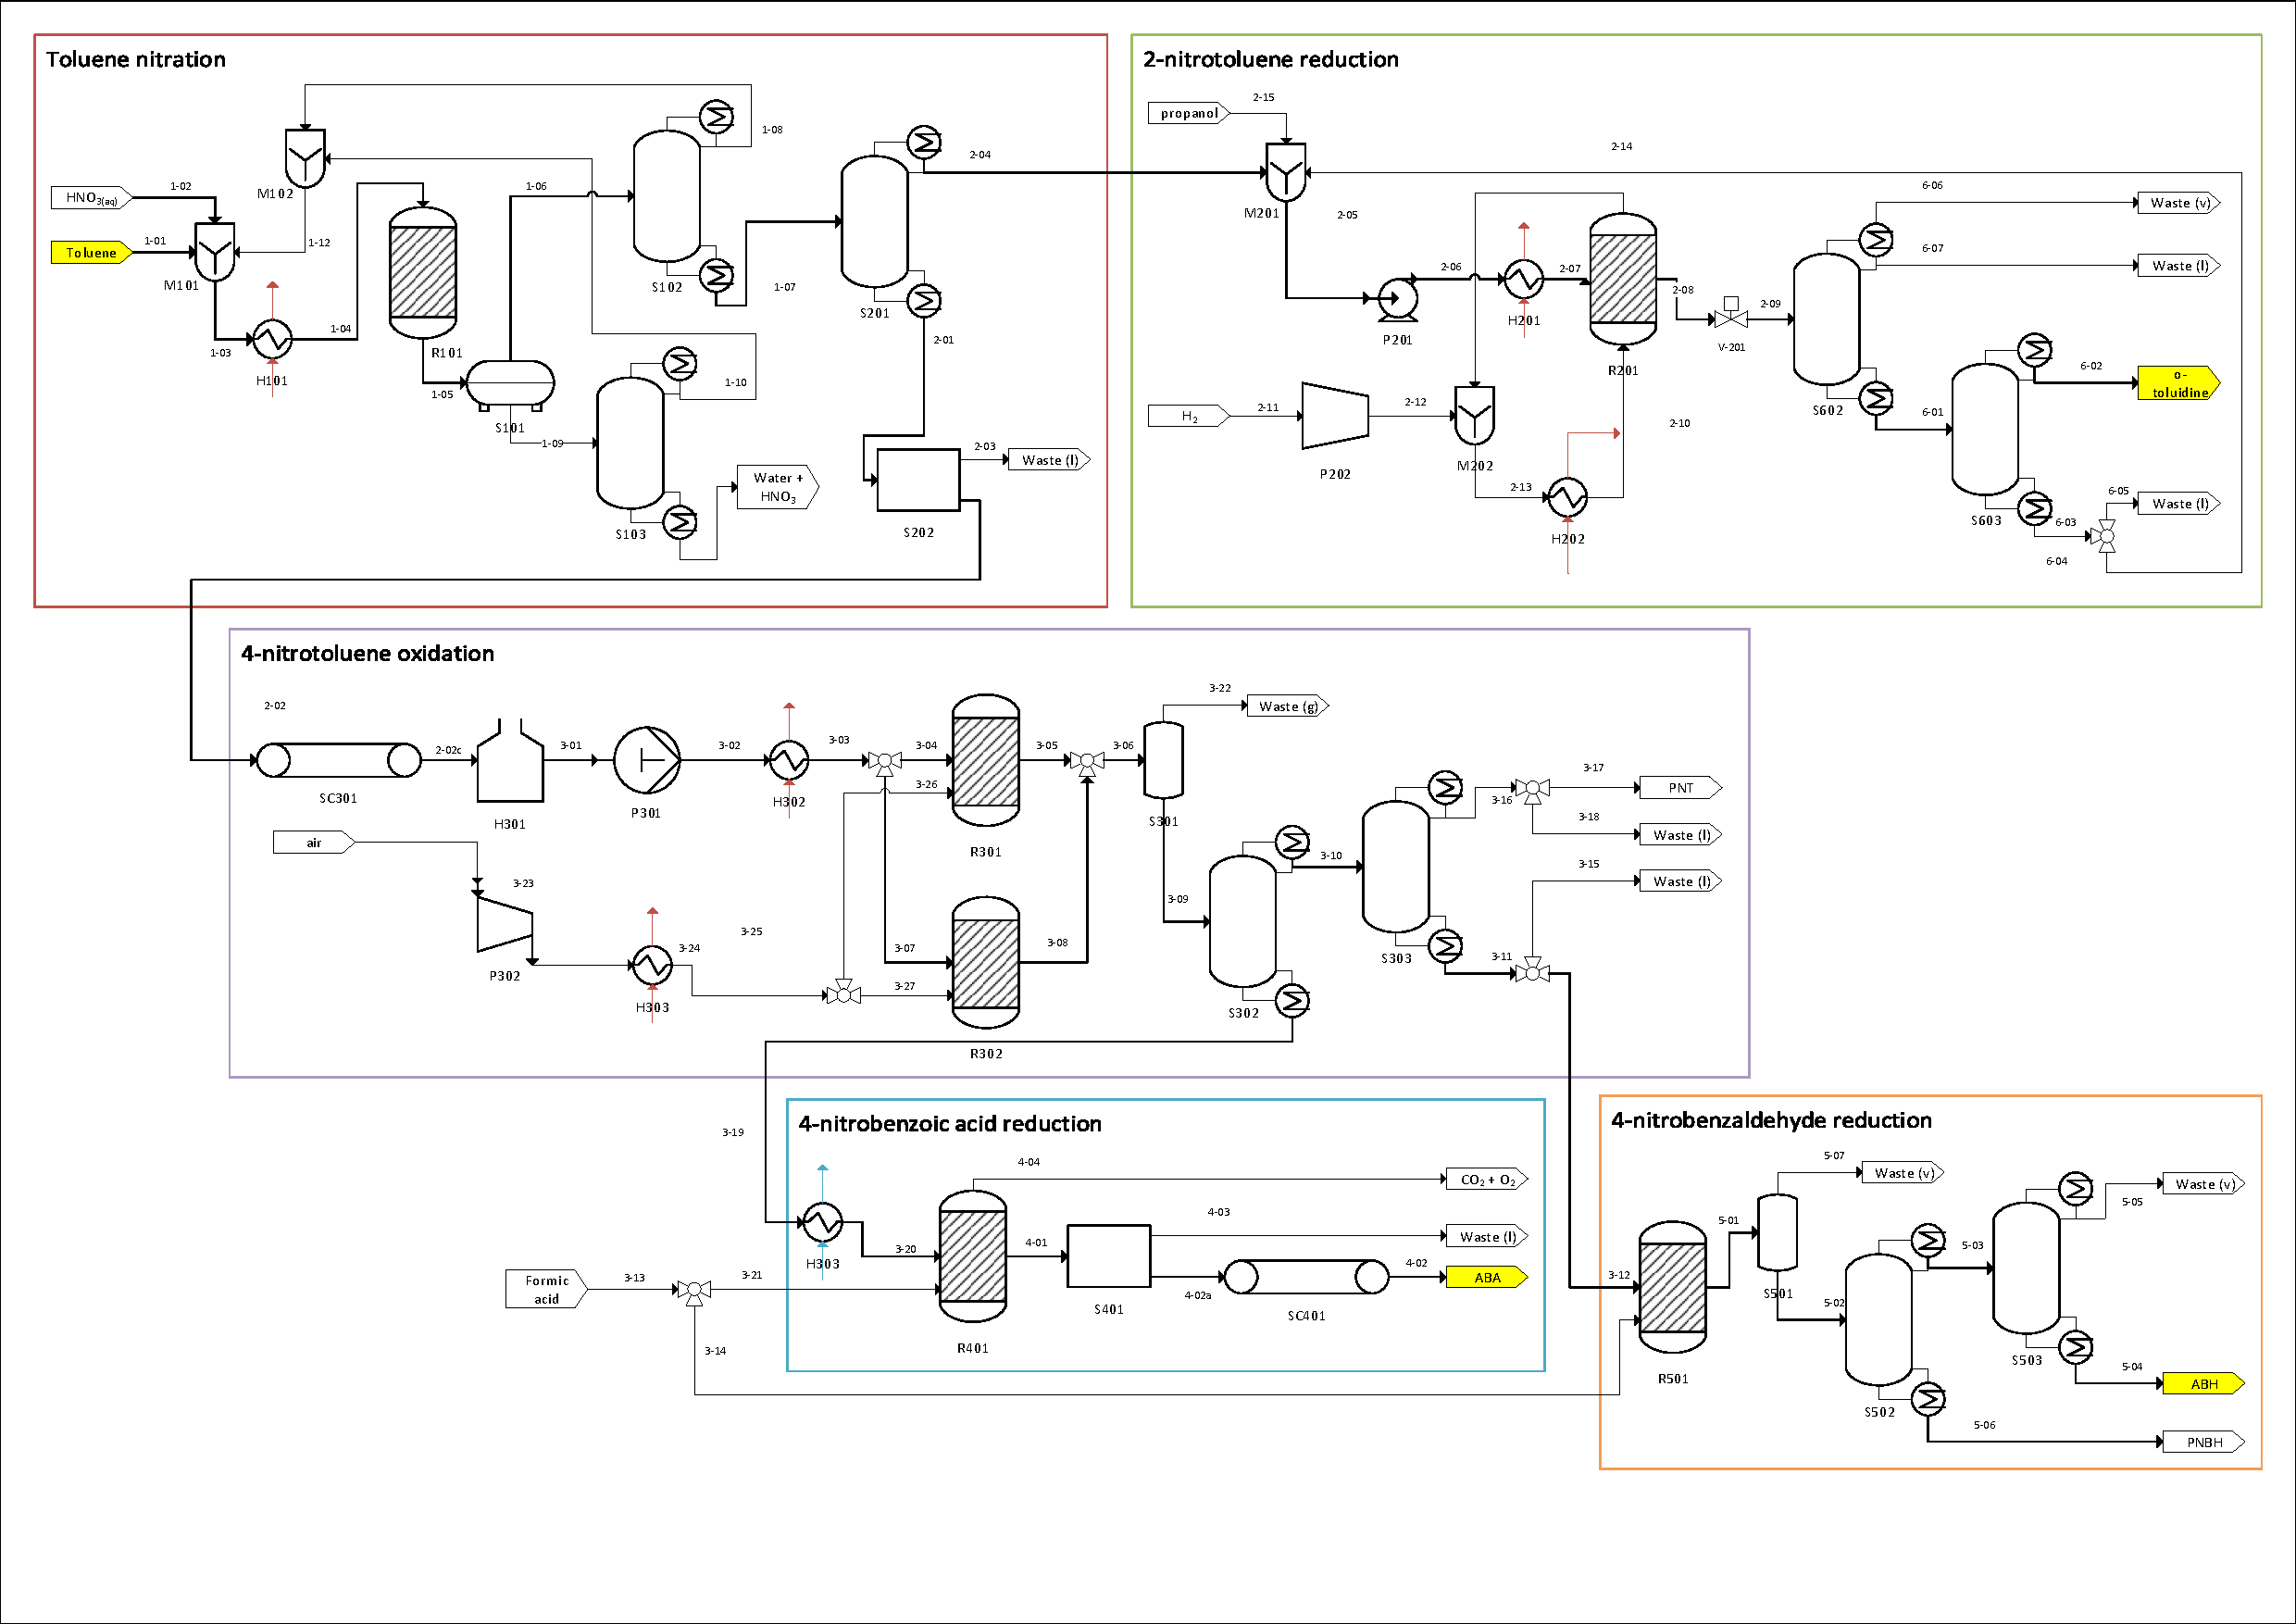
\includepdf[pages=-,landscape,fitpaper]{figures/NitromaPFD-2021-02-07.pdf}

% !TeX root = ../main.tex
\begin{landscape}


\section{Stream Tables}
\label{app:drawings}
\end{landscape}

% !TeX root = ../main.tex
\section{Decision Analysis}
\label{app:matrix}

\subsection{Sample AHP and TOPSIS calculation for product selection}

\paragraph{1. Pair-wise comparison of criteria}
The scale developed by Saaty was adopted to assess the relative importance of one criteria to another \cite{saaty_analytic_1987}. The fundamental scale is as follows: 1 for equal importance, 3 for moderate importance of one criteria over the other, 5 for essential or strong importance, 7 for very strong importance and 9 for extreme importance. Even numbers can be used as intermediate values. The normalised weightings were then calculated. The results for product selection are shown in \Cref{tab:pairwise}. Environmental and safety considerations were valued has more important than other criteria, in line with Nitroma's commitment to develop an inherently safer process. Process complexity was given the lowest weighting since each route exhibited similar complexities to achieve a multipurpose plant.  

\begin{table}[H]
\centering
\caption{Pair-wise criteria comparison for product selection}
\label{tab:pairwise}
\begin{tabularx}{\linewidth}{l|XXX|l}
\toprule
                                                                & Economic potential & Process complexity & \splitcell{Environmental\\ and safety} & Weights \\ \midrule
Economic potential                        & 1.000              & 3.000              & 0.333                    & 0.286   \\
Process complexity                      & 0.333              & 1.000              & 0.333                    & 0.14    \\
Environmental and   safety & 3.000              & 3.000              & 1.000                    & 0.574   \\ \midrule
Sum                                      & 4.333              & 7.000              & 1.667                    &                              \\ \bottomrule
\end{tabularx}
\end{table}


\paragraph{2. Validation of consistency}
The consistency between the weightings was verified with a method proposed by Saaty \cite{saaty_analytic_1987}. The largest eigenvalue ($\lambda_{max}$) was determine with the following formula where $i$ refers to the criteria:
\begin{equation}
    \lambda_{max}=\sum^{i} \mathrm{w}_{i}\cdot \mathrm{Sum}(i)
\end{equation}
The consistency index (CI) is calculated for the number of criteria $n$:
\begin{equation}
   \mathrm{CI} = \frac{\lambda_{max}-n}{n-1}
\end{equation}
The consistency ratio CI/RI is then calculated using the Random Consistency Index (RI) retrieved from (Saaty, 1987). 
For product selection, $\lambda_{max}$=3.036, CI=0.018 and RI=0.58, hence the consistency ratio is worth 0.03. Weightings are deemed consistent if the ratio is less than 10\%.\\

\paragraph{3. AHP score calculation}
The score for a given alternative is calculated by summing, over all criteria, the normalised score multiplied by the criteria weighting:
\begin{equation}
    S=\sum^{i}_{n}(\tilde{p}_{in} \cdot w_{i})
\end{equation}

\paragraph{4. Weighted Normalised Matrix for TOPSIS}
Similarly to AHP analysis, a $n\times k$ matrix is constructed for $n$ criteria and $k$ alternatives. The criterion $X_{ij}$ are normalised and multiplied by their respective weighting $w_i$ as follows:
\begin{align}
    \tilde{X}_{ij}&=\frac{X_{ij}}{\sqrt{\sum^{n}_{i=1}X_{ij}^{2}}} &
    V_{ij}&=\tilde{X}_{ij}\times w_j
\end{align}

\paragraph{5. Calculation of Euclidean distance from ideal best and ideal worst}
The ideal best and ideal worst are the maximum and mimnim values for each criterion. The distance of each criterion to the ideal best ($V_{j}^{+}$) and ideal worst ($V_{j}^{-}$) values is calculated as follows:
\begin{align}
    S_{i}^{+}&=\sqrt{\sum_{j=1}^{n}(V_{ij}-V_{j}^{+})^2} &
    S_{i}^{-}&=\sqrt{\sum_{j=1}^{n}(V_{ij}-V_{j}^{-})^2}
\end{align}

\paragraph{6. Evaluation of Performance Score and ranking}
Finally the performance score is the ratio between the Euclidian distance from the ideal worst and the sum of Euclidian distances. The highest score indicates the most optimum solution.
\begin{equation}
    P_{i}=\frac{S_{i}^{-}}{S_{i}^{+}+S_{i}^{-}}
\end{equation}



\subsection{Nitration catalyst selection}

\begin{table}[h]
\centering
    \caption{AHP/TOPSIS results for nitration catalyst selection}
    \label{tab:nitration}\footnotesize
\begin{tabular}{l|S[table-format=2.3]S[table-format=1.2]|S[table-format=2.0]|lll|S[table-format=1.3]S[table-format=1.3]c}
\toprule
                                          & \multicolumn{2}{c|}{Economic potential   (14\%)}                                & {Performance (57\%)} & \multicolumn{3}{c|}{EHS (29\%)}     &                       &                          &                           \\ \cmidrule{2-7}
                                          & {\splitcell{Price\\(\si{\EUR\per\g})}} & {\splitcell{By-products\\(\%)}} & {Conversion (\%)}  & \rotatebox[origin=r]{90}{Health} & \rotatebox[origin=r]{90}{Flammability} & \rotatebox[origin=r]{90}{Instability} & AHP & TOPSIS & Rank \\ \midrule
H-ZSM-5 & 0.734        & 0.5 & 41                             & 2       &  0          &     0       & 0.297                 & 0.752                & 2                         \\ 
H-Y & 0.696            & 0.48 & 36                           & 2      &        0     & 0           & 0.276                 & 0.705                   & 3 \\ 
H-Mordenite       & 0.726           & 0.55  & 43                            & 2      &     0        & 0           & 0.303                 & 0.761                  & \cellcolor{green}1 \\ 
No catalyst         & 0            & 0 & 2                         & 0      & 0            & 0           & 0.124                 & 0.237                    & 4                         \\ 
\bottomrule
\end{tabular}
\end{table}




\subsection{Solvent for 2-nitrotoluene hydrogenation}
\begin{table}[h]
\centering
    \caption{AHP/TOPSIS results for o-nitrotoluene hydrogenation solvent selection}
    \label{tab:solvent}\footnotesize
\begin{tabularx}{\linewidth}{l|X|S[table-format=2.2]S[table-format=1.2]S[table-format=1.3]|ll|llll|S[table-format=1.3]S[table-format=1.3]c}
\toprule
                                          & Economic potential   (11\%)                                & \multicolumn{3}{c|}{Performance (24\%)} & \multicolumn{2}{c|}{\splitcell{Safety\\ (52\%)}}     & \multicolumn{4}{c|}{Sustainability (13\%)}                        &                          &                           \\ \cmidrule{2-11}
                                          & \splitcell{Price\\ (\si{\GBP\per\L})} & {\splitcell{Activation\\ energy\\ (\si{\kJ\per\mol})}} & {\splitcell{Reaction\\ rate\\  (\si{\mol\per\s})}}  & {\splitcell{\ch{H2} solubility\\ (\si{\mL\of{\ch{H2}}\per\mL\of{solution}})}}& \rotatebox[origin=r]{90}{Health} & \rotatebox[origin=r]{90}{Flammability} & \rotatebox[origin=r]{90}{Renewability} & \rotatebox[origin=r]{90}{Environment} & \rotatebox[origin=r]{90}{Waste} & \rotatebox[origin=r]{90}{LCA} & AHP & TOPSIS & Rank \\ \midrule
Methanol & 28.6       & 34.36 & 2.14     & 0.809       &  5          &     5      & 3 & 9 & 4 & 9 & 0.212                 & 0.531                & 2                        \\ 
Propanol & 39           & 45.52 & 1.34  & 0.825     &        6     & 8           & 2 & 9 & 3 & 4 & 0.213                 & 0.707                   & \cellcolor{green}1 \\ 
Butanol      & 47.8         & 50.08  & 1.31      & 0.844      &     8        & 6    & 3 & 7 & 5 & 5       & 0.211                & 0.701                  & 3 \\ 
Cyclohexanol       & 37.6            & 60.48 & 0.51   & 0.325      & 9            & 7      & 1 & 6 & 6 & 8     & 0.207                & 0.631                    & 4                        \\ 
Hexane     & 60           & 66.21 & 1.29      &   1.981    & 2            & 4 & 1 & 3 & 5 & 7         & 0.157                 & 0.362                    & 5                        \\ 
\bottomrule
\end{tabularx}
\end{table}

\subsection{Plant location}


\begin{table}[H]
\centering
    \caption{AHP/TOPSIS results for plant location selection}
    \label{tab:location selection}\footnotesize
\adjustbox{max width=\textwidth}{
\begin{tabular}{l|ll|lll|ll|lll|l|l|llc}
%S[table-format=2.2]S[table-format=1.2]S[table-format=1.3]
\toprule
                                          & \multicolumn{2}{c|}{\splitcell{Supply chain\\ (34\%)}}                               & \multicolumn{3}{c|}{\splitcell{Country economics\\ (17\%)}} & \multicolumn{2}{c|}{\splitcell{Trade\\ (4\%)}}     & \multicolumn{3}{c|}{Operating costs (28\%)}   & \splitcell{Competitive\\ Landscape (9\%)} & \splitcell{Political\\ stability (7\%)}  &     &                      \\ \cmidrule{2-13}
                                          
                                      & {\rcell{Local toluene production (\si{\tonne\per\year})}} & {\rcell{Industry size of products (\si{\USD b})}} & \rtext{Interest rate (\%)}  & \rcell{Corporate tax rate (\%)} & \rtext{Inflation (\%)} & \rtext{Import duties (\%)} & \rtext{Export duties (\%)} & {\rcell{Electricity cost (\si{\USD\per\kWh})}} & {\rcell{Minimum wage (\si{\USD\per\h})}} & {\rcell{Cooling water cost (\si{\USD\per\l})}} &  {\rcell{Number competitors}} & {\rcell{Corruption perception index}} & AHP & TOPSIS & Rank \\ \midrule
India & 1       & 20 & 4     & 7.35       &  7.35          &     4.9      & 7.5 & 0.08 & 1.00 & 0.2 & 2                 & 41                & 0.193 & 0.536 &    3              \\ 
China & 1          & 95 & 3.85  & 6.5     &       1.6     & 3.4           & 6.5 & 0.08 & 1.68 & 0.33 & 48                 & 41                 & 0.284 & 0.922 & \cellcolor{green}1  \\ 
USA     & 1        & 501  & 0.25      & 5.25      &     1.2        & 1.6    & 5.25 & 0.15 & 7.30 & 1.53       & 157               & 69                 & 0.218 & 0.659 & 2 \\ 
Germany      & 1            & 47 & 0   & 6.5      & -0.3            & 1.7      & 6.5 & 0.38 & 10.97 & 2.46     & 33               & 80                   & 0.182         & 0.485 &  4          \\ 
Poland    & 1           & 7.9 & 0.1      &   6.5   & 12.6            & 2.5 & 6.5 & 0.19 & 3.35 & 0.93         & 0                 & 39                  &    0.123         & 0.290 &     5      \\ 
\bottomrule
\end{tabular}
} % adjustbox
\end{table}
% !TeX root = ../main.tex
\section{Unit Sizing Methodology}
\label{app:sizing}
\subsection{Reactor Sizing}
%Based on X paper, (include why reactors are PFR) (reference Levenspiel)

All the reactors used in Nitroma's plant are assumed to have the same design equation as a plug flow reactor:
\begin{equation}
    V_R = \int_{F_{A0}}^{F_{A}} \frac{\dd F_A}{-r_A} = \int_{F_{A0}}^{F_{A}} \frac{\dd F_A}{-kC_A}
    \label{reactor_sizing}
\end{equation}
The plug flow behaviour is a common assumption for packed-bed reactors, ignoring axial and radial dispersion \cite{froment_chemical_nodate}. Similarly, studies have shown that  trickle bed reactor also behaves as an ideal plug flow reactor with no interphase and intraparticle gradients \cite{p_a_ramachandran_recent_1987}.

\paragraph{Key assumptions}
\begin{enumerate}
    \item Using the rate equation in the design equation accounts for intrinsic kinetics but not for mass transfer limitations when sizing the reactor. The effects of mass transfer limitations on the rate might be significant for the hydrogenation of ONT to o-toluidine as the rate is dependent on the catalyst. Including the effectiveness factor in the rate equation will provide a more accurate representation of the volume, but these limitations are not considered at this stage.
    \item Catalysts are used in all of the designed reactors. For more accurate sizing of the reactors, the deactivation of the catalyst should be reflected in the rate equation given by the deactivation function. The catalysts used in the reactors have a relatively long deactivation time \cite{temizel_novel_2020}, so the deactivation of the catalysts is considered to be negligible at this stage.
\end{enumerate}

\subsection{Separator Unit Sizing}
Summary of the key assumptions involved in sizing the separator units and their sources of reference are listed in Table \ref{tab:assumptions of sizing separator units} below. 

\begin{table}[h]
\centering\small
    \caption{Key assumptions involved in sizing of separator units and their sources of reference}
    \label{tab:assumptions of sizing separator units}\footnotesize
\begin{tabularx}{\linewidth}{llXl}
\toprule
Tag  & Type                 & Assumptions used in sizing                                                                                                                                      & Source                                             \\ \midrule
S101 & Decanter             & Aqueous phase is continuous; organic phase is dispersed                                                                                                         & \cite{ludwig_applied_1994}                         \\
S102 & Distillation column  & Diameter of plate column estimated using methodology proposed in Seider et al. 2009; height to diameter ratio designed to be 25 in accordance with Douglas 1988 & \cite{seider_product_2009,douglas_conceptual_1988} \\
S103 & Distillation column  & Diameter of plate column estimated using methodology proposed in Seider et al. 2009; height to diameter ratio designed to be 25 in accordance with Douglas 1988 & \cite{seider_product_2009,douglas_conceptual_1988} \\
S201 & Distillation column  & Diameter of plate column estimated using methodology proposed in Seider et al. 2009; height to diameter ratio designed to be 25 in accordance with Douglas 1988 & \cite{seider_product_2009,douglas_conceptual_1988} \\
S202 & Crystalliser         & No wetting (pure solid crystals); scaling by solid production rate from past example (Sulzer falling-film melt crystalliser)                                    & \cite{seader_separation_2011}                      \\
S301 & Flash drum           & Minimum residence time of liquid phase is \SI{5}{\minute}; vessel half-filled with liquid                                                                                 & \cite{seader_separation_2011}                      \\
S302 & Distillation column  & Diameter of plate column estimated using methodology proposed in Seider et al. 2009; height to diameter ratio designed to be 25 in accordance with Douglas 1988 & \cite{seider_product_2009,douglas_conceptual_1988} \\
S303 & Distillation column  & Diameter of plate column estimated using methodology proposed in Seider et al. 2009; height to diameter ratio designed to be 25 in accordance with Douglas 1988 & \cite{seider_product_2009,douglas_conceptual_1988} \\
S401 & Crystalliser         & No wetting (pure solid crystals); scaling by solid production rate from past example (Sulzer falling-film melt crystalliser)                                    & \cite{seader_separation_2011}                      \\
S501 & Flash drum           & Minimum residence time of liquid phase is \SI{5}{\minute}; vessel half-filled with liquid                                                                                 & \cite{seader_separation_2011}                      \\
S502 & Distillation column  & Diameter of plate column estimated using methodology proposed in Seider et al. 2009; height to diameter ratio designed to be 25 in accordance with Douglas 1988 & \cite{seider_product_2009,douglas_conceptual_1988} \\
S503 & Distillation column  & Diameter of plate column estimated using methodology proposed in Seider et al. 2009; height to diameter ratio designed to be 25 in accordance with Douglas 1988 & \cite{seider_product_2009,douglas_conceptual_1988} \\
S601 & Distillation  column & Diameter of plate column estimated using methodology proposed in Seider et al. 2009; height to diameter ratio designed to be 25 in accordance with Douglas 1988 & \cite{seider_product_2009,douglas_conceptual_1988} \\
S602 & Distillation  column & Diameter of plate column estimated using methodology proposed in Seider et al. 2009; height to diameter ratio designed to be 25 in accordance with Douglas 1988 & \cite{seider_product_2009,douglas_conceptual_1988} \\ \bottomrule
\end{tabularx}
\end{table}

\noindent Detailed methodologies for the sizing are as following:

\paragraph{Distillation columns}
The distillation columns have been designed following the method outlined in \textcite{seider_product_2009}.
\begin{equation}
    D_t = \left[\frac{4G}{(fU_f)\pi\left(1-\frac{A_d}{A_T}\right)\rho_g}\right]^\frac{1}{2}
    \label{distill_dia_sizing}
\end{equation}
where G is the vapour mass flowrate, $fU_f$ is the fraction of the flooding velocity, $\frac{A_d}{A_T}$ is the ratio of downcomer area to the cross sectional area of the tower and $\rho_g$ is the mass density of the vapour.
Column heights were calculated by using a general rule quoted in \textcite{douglas_conceptual_1988} that the height should be 20-30 times the diameter of the column, to prevent buckling under strong winds if too tall so a ratio of 25 was taken. 
\begin{equation}
    H_t = 25D_t
    \label{distill_height_sizing}
\end{equation}

\paragraph{Crystallisers}
The crystallisers in this design have been sized by scaling against a past example of falling-film melt crystalliser develped by Sulzer Brothers Ltd. According to \textcite{seader_separation_2011} this equipment produces high-purity crystals at a capacity of \SI{100000}{\tonne\per\year}; it consists of a pair of units \SI{4}{\m} in diameter and \SI{12}{\m} in height. By assuming in this design that the solid crystals are pure and no wetting occurs, we scaled the crystalliser by its solid production rate as shown in Equation \ref{crystalliser_sizing} below:
\begin{equation}
    V = \frac{S}{\SI{10000}{\tonne\per\year}} \times 2~((\frac{4}{2}~m)^2 \pi \times 12~m)
    \label{crystalliser_sizing}
\end{equation}
where $V$ is the volume of the crystalliser and $S$ is the solid production rate in \si{\tonne\per\year}.

\paragraph{Flash drums}
According to \textcite{seader_separation_2011} the minimum volume of a vertical reflux/flash drum is to be determined on the basis of liquid residence time; the liquid residence time should be at least \SI{5}{\minute} and half of the vessel is assumed to be filled with liquid. Thus, Equation \ref{flash_sizing} below can be used to estimate the volume of the flash drum:
\begin{equation}
    V = \frac{2 L M_L t}{\rho_{L}}
    \label{flash_sizing}
\end{equation}
where $V$ is the volume of the flash drum, $L$ is the molar liquid flow rate leaving the vessel, $M_L$ is the average molecular weight of the liquid, $t$ is the minimum residence time, and $\rho_L$ is the average molar density of the liquid. 
% !TeX root = ../main.tex
\section{Process alternatives}
\label{app:alternatives}

\subsection{Mixed-acid nitration}
\label{mixed}

\subsection{Nitration reactor}
\label{nitrationreactor}
\subsubsection{Packed-bed reactor}
A conventional packed-bed reactor was considered for the nitration process. This reactor is easy to operate because the packed structure of the catalyst removes the need for catalyst filtration in the outlet stream . The compact catalyst packing also allows for high zeolite catalyst loading []. A simple modelling of a packed-bed reactor usually assumes perfect mixing, however, in reality flow maldistribution and hot spot formation occurs []. This is dangerous for the nitration process as any hot spots will promote the thermal runaway process that increases the risk of explosion. Therefore, to increase the inherent safety of Nitroma's plant, this option was not pursued further.

\subsubsection{Slurry reactor}

\subsection{Toluidine hydrogenation reactor}
\label{toluidine}
\subsubsection{Stirred Slurry reactor}
An alternative reactor for toluidine hydrogenation was the slurry reactor. Attrition of the solid Pd catalyst will occur in slurry reactors due to the violent agitation in the reactor, damaging the catalyst. As Pd catalyst is considered as a precious metal, catalyst regeneration will be very expensive thus lowering the EP of this plant. A slurry reactor was more applicable for a lower pressure reaction, as 

was not applicable for a high pressure operations like this due to the mechanical parts and difficult
, thus this option was eliminated. []


\subsection{Direct 4-aminobenzaldehyde production}
\label{direct}
% !TeX root = ../main.tex
\section{Kinetics Parameters}
\label{app:kinetics}

%\subsection{Summary of production routes}

% 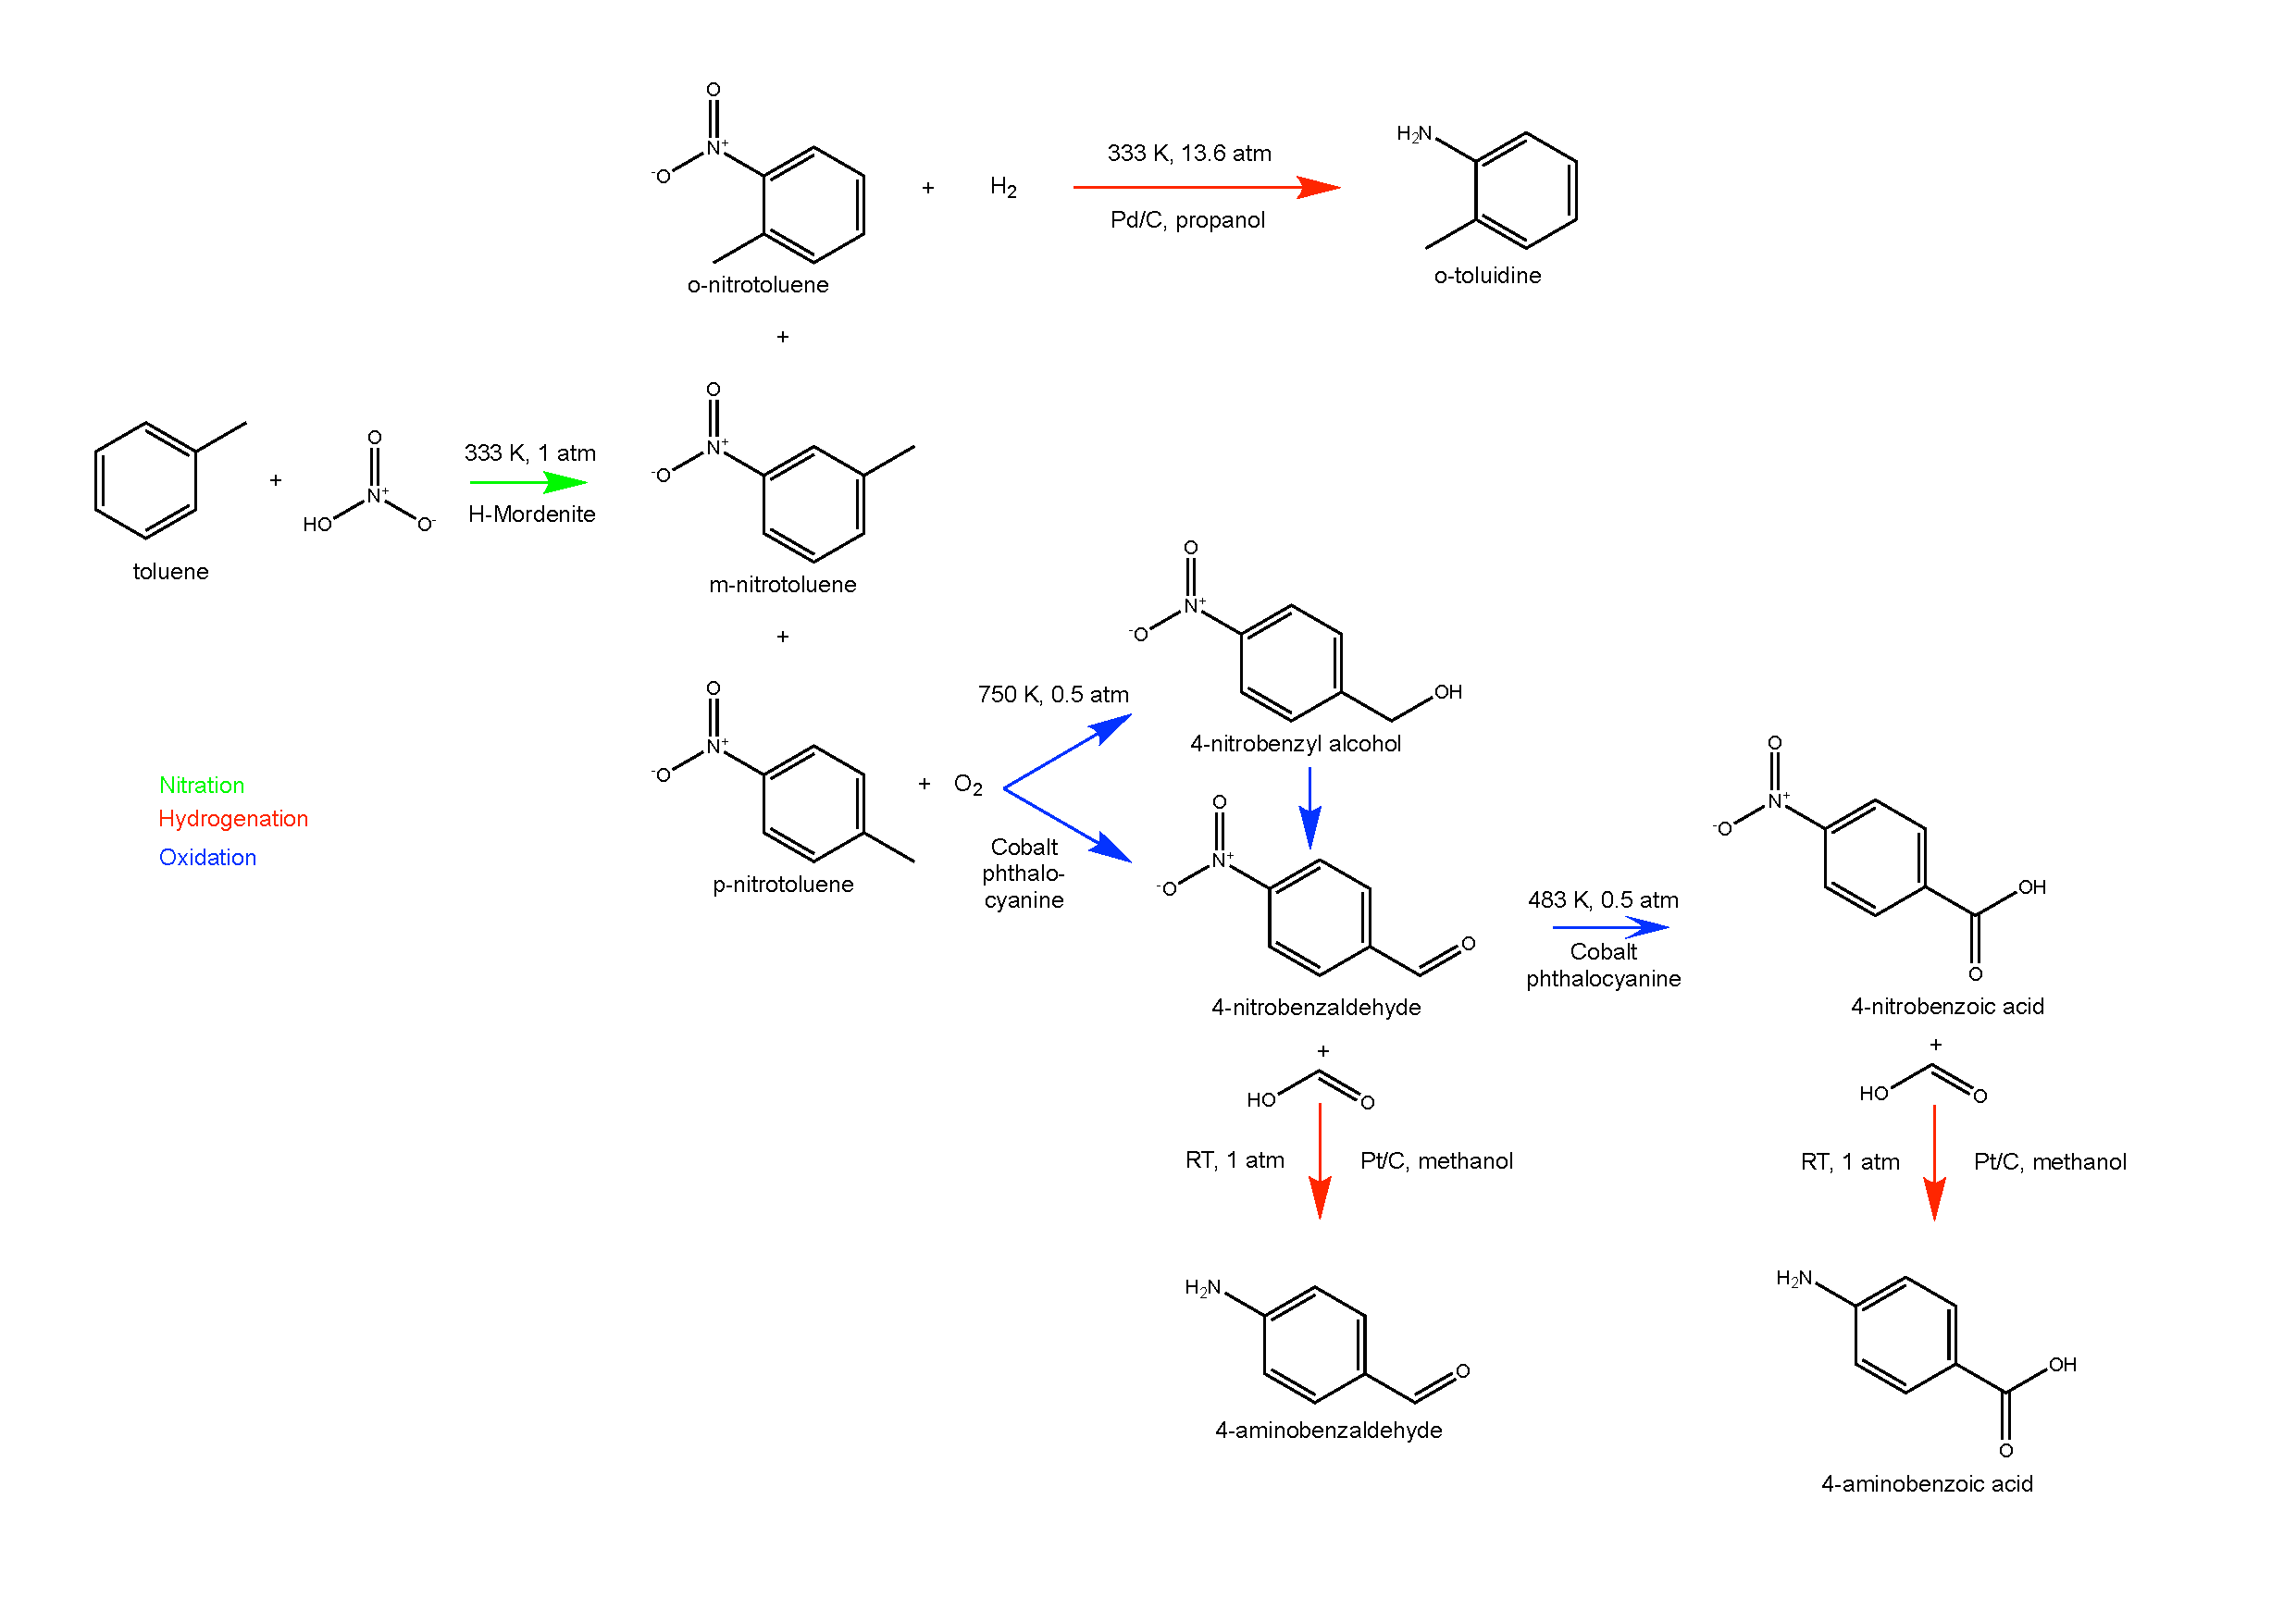
\includepdf[pages=-,landscape]{figures/routes-chosen.pdf}

\afterpage{
\begin{landscape}
\begin{figure}[H]
    \centering
    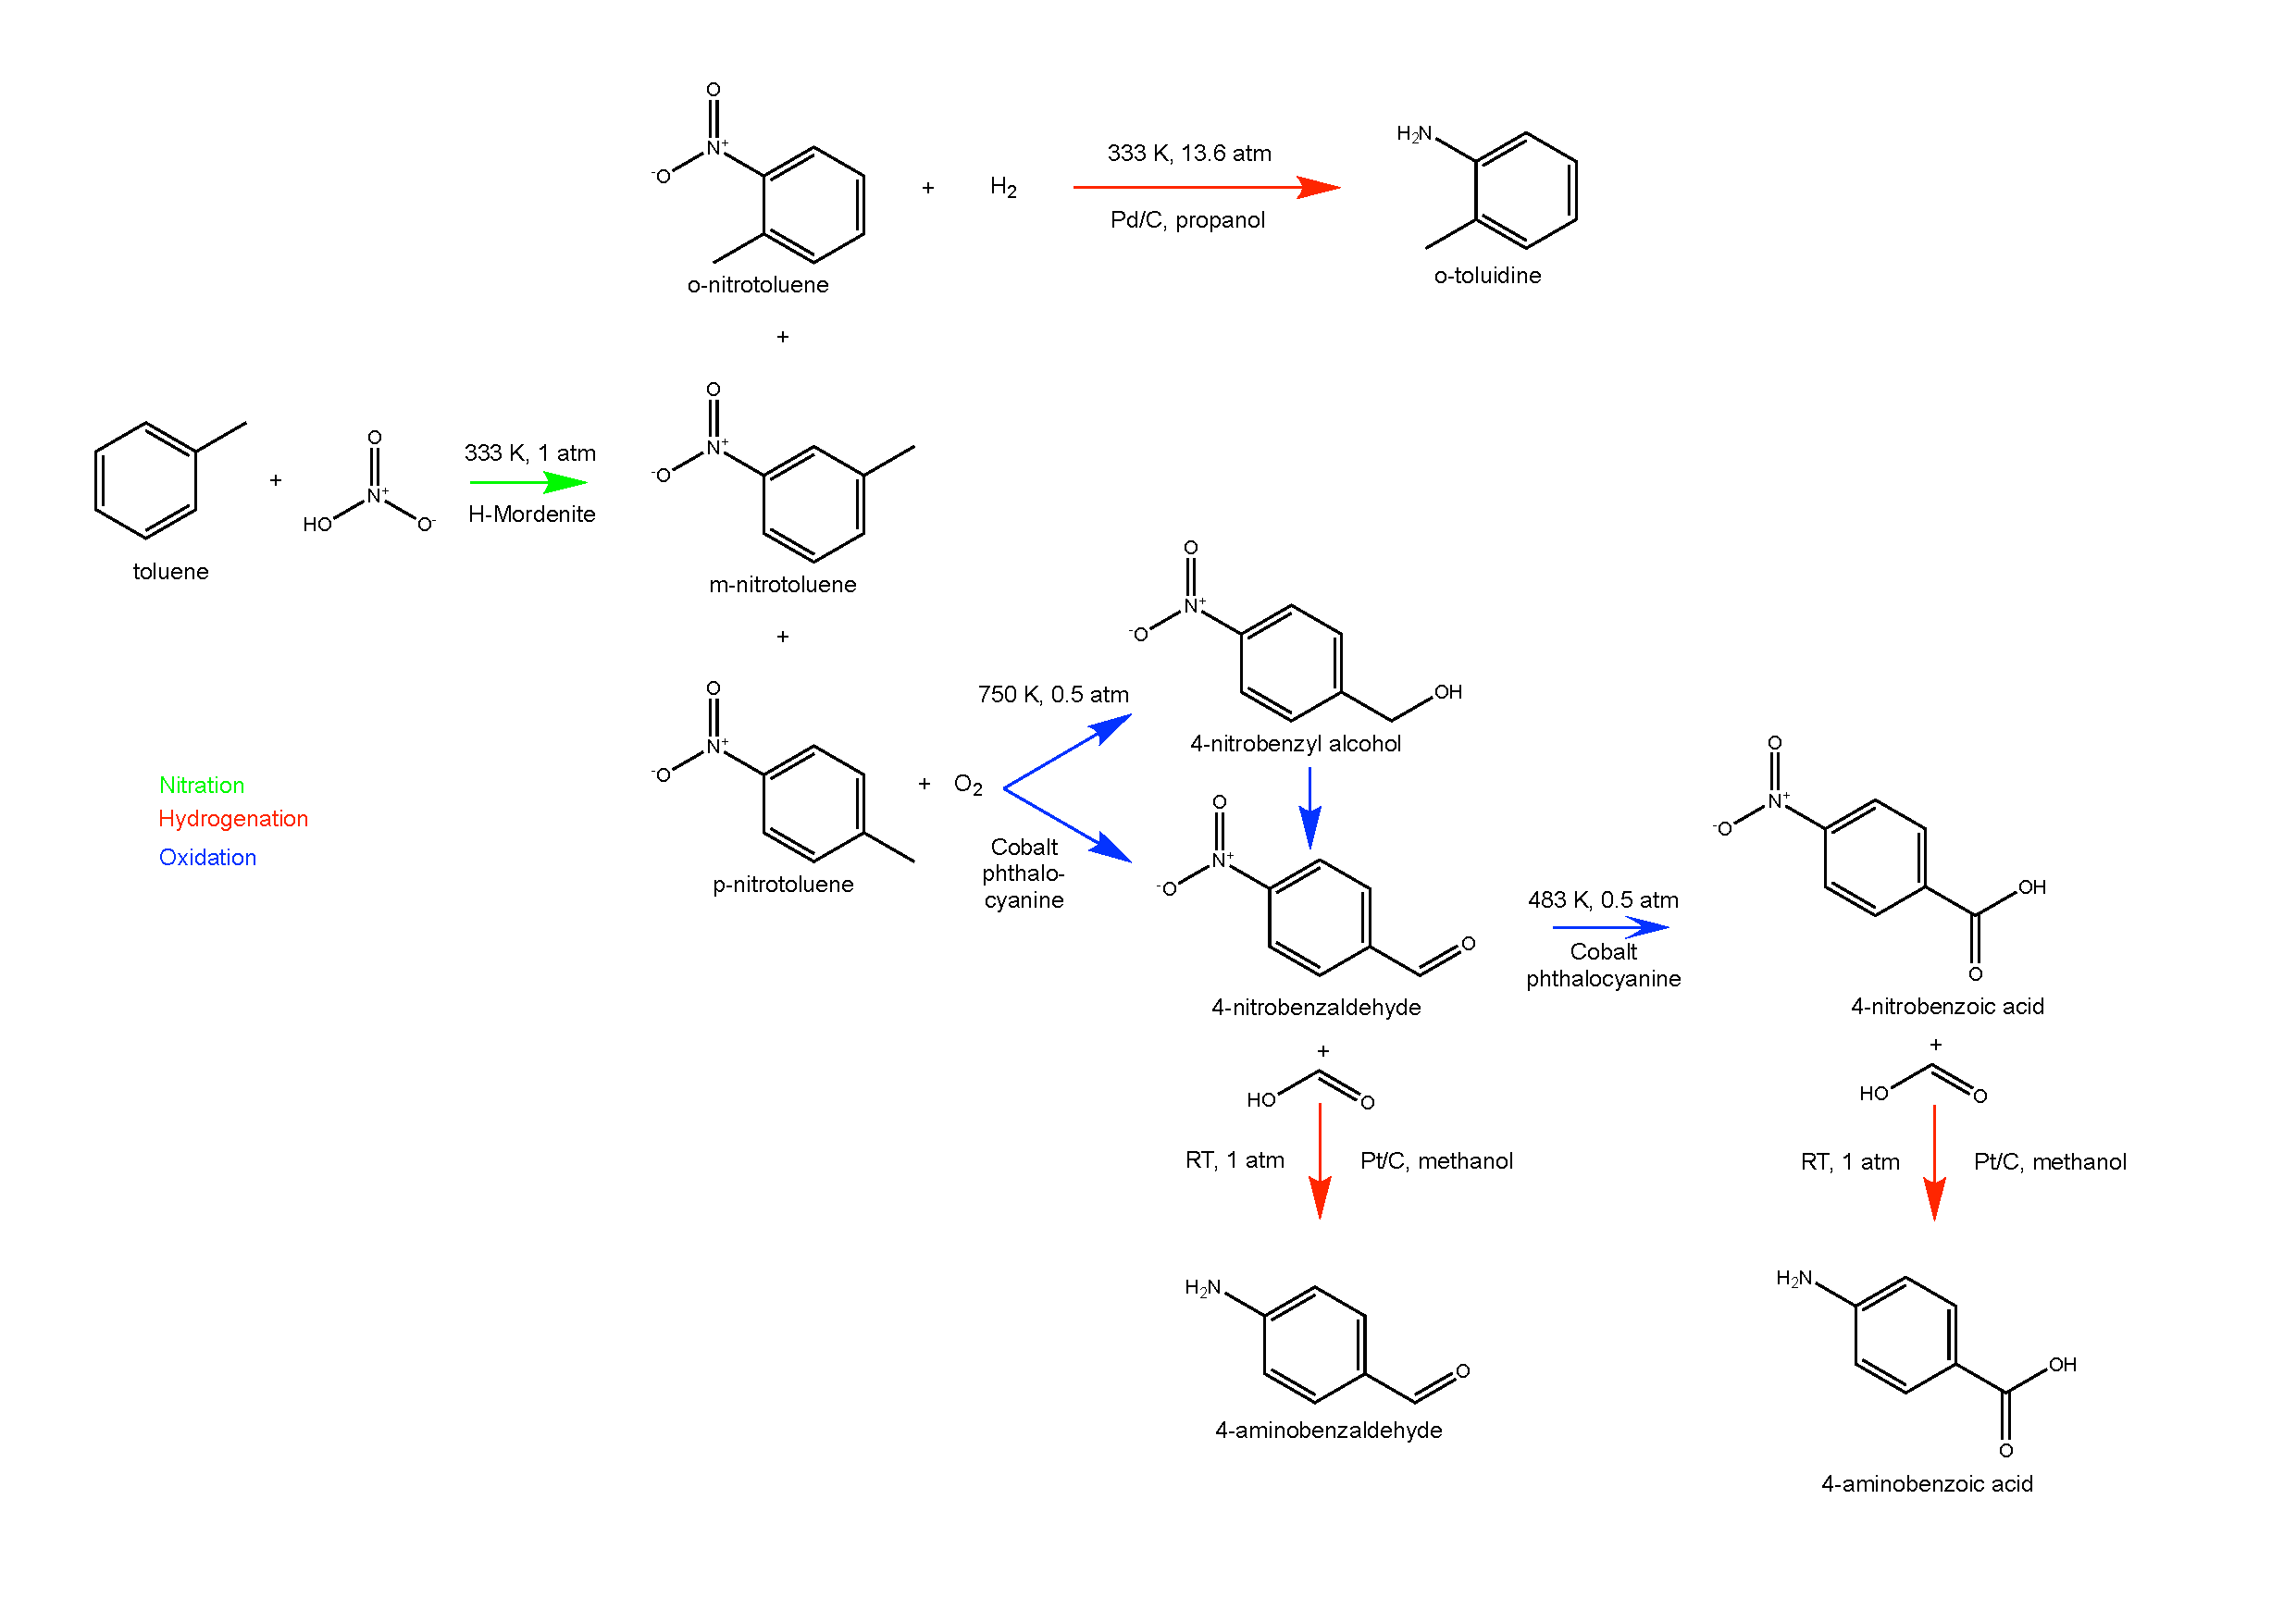
\includegraphics[width=0.8\linewidth]{figures/routes-chosen.pdf}
    \caption{Selected synthesis routes}
    \label{fig:routes-chosen}
\end{figure}
\end{landscape}
}

\subsection{Toluene nitration}
\paragraph{Assumptions}
\begin{itemize}
    \item The stoichiometric reaction is \ch{Toluene +  HNO3 -> 0.44 PNT + 0.03 MNT + 0.53 ONT + H2O}, where PNT, MNT and ONT are respectively the \textit{para}, \textit{meta} and \textit{ortho} isomers of nitroltoluene.
    \item The ratio of isomers is reflected in the stoichiometric eqution \cite{smith_novel_1998}.
    \item Negligible production of dinitrotoluene by-products as reported selectivity with H-Mordenite catalyst is lower than 0.55mol\% \cite{jeeru_kinetics_2018}.
    \item Kinetic parameters were obtained for a system free from mass transfer resistances and thus when the reaction is kinetically controlled \cite{jeeru_kinetics_2018}. Hence we can safely assume that the intrinsic rate of reaction was measured.
    \item The rate of reaction of toluene is first order in toluene and nitric acid concentrations. However with 2:1 mole ratio of nitric acid to toluene, the rate can be approximated to a pseudo-first order reaction with respect to toluene \cite{jeeru_kinetics_2018}.
    \begin{equation}
    - \frac{dC_{toluene}}{dt}=k \cdot C_{toluene} 
    \end{equation}
    \item The rate constant follows the Arrhenius law below, which is valid for a reaction temperature range of 303-363K \cite{jeeru_kinetics_2018}:
    \begin{equation}
        k=2.5e^{-\frac{24.24\cdot 10^{3}}{RT}}
    \end{equation}
    \item The loss in activity of the catalyst can be neglected \cite{jeeru_kinetics_2018}.
\end{itemize}

\subsection{o-nitrotoluene hydrogenation}
\paragraph{Assumptions}
\begin{itemize}
    \item The stoichiometric reaction is \ch{ONT +  3 H2 -> \ortho-toluidine + 2 H2O} \cite{zhao_new_2016}.
    \item Negligible production of toluene and aniline by-products.  
    \item The side-chain alkylation of ONT can be avoided, thus no nitrostyrene and nitroethylbenzene can be formed \cite{zhao_new_2016}.
    \item Kinetic parameters were obtained for a system free from mass transfer resistances and are thus the intrinsic rate of reaction.
    \item The rate of reaction of ONT is 0.3 order with respect to hydrogen pressure and depends on the mass of Pd/C catalyst \cite{rajadhyaksha_solvent_1986}:
    \begin{equation}
    - \frac{dC_{ONT}}{dt}=k \cdot P_{\ch{H2}}^{0.3} 
    \end{equation}
    \item The rate constant, in mol/(kPa$^{0.3}$g$_{cat}$s), is valid for a reaction temperature range of 333-363K \cite{rajadhyaksha_solvent_1986}:
    \begin{equation}
        k=211e^{\frac{-45.52\cdot 10^{3}}{RT}}
    \end{equation}
    \item The loss in activity of the catalyst is neglected.
\end{itemize}

\subsection{4-nitrotoluene oxidation}
\paragraph{Assumptions}
\begin{itemize}
    \item Nitrotoluene follows the same reaction pathways as toluene \cite{wendt_reaction_1986}.
    \item The stoichiometric reactions are as follow \cite{hoorn_modelling_2005}:
    \begin{enumerate}
        \item \ch{PNT +  O2 -> NBH + H2O}
        \item \ch{PNT +  0.5 O2 -> NBO}
        \item \ch{NBH +  0.5 O2 -> NBA}
        \item \ch{NBO +  0.5 O2 -> NBH + H2O}
    \end{enumerate}
    \item The reactivity of nitrotoluene and derivatives, and thus the reaction rates, are 5.6 times slower than for toluene \cite{partenheimer_methodology_1995}.
    \item Kinetic parameters were obtained for a system free from mass transfer resistances and thus when the reaction is kinetically controlled \cite{chandalia_kinetics_1999}. Hence we can safely assume that the intrinsic rate of reaction was measured.
    \item Reaction is independent of the oxygen partial pressure for high oxygen concentrations \cite{tan_kinetic_2010}.
    \item The reactions are first order with respect to the aromatic concentration \cite{chandalia_kinetics_1999}.
    \item The rate constants, in \si{\per\s}, follow the Arrhenius law \cite{tan_kinetic_2010}:
        \begin{align}
            k_1&=7.068 \times 10^9 e^{-\frac{123.91\cdot 10^{3}}{RT}}\\
            k_2&=1.503 \times 10^3 e^{-\frac{69.54 \cdot 10^{3}}{RT}}\\
            k_3&=5.621 \times 10^4 e^{-\frac{66.84 \cdot 10^{3}}{RT}}\\
            k_4&=3.384 \times 10^6 e^{-\frac{81.27 \cdot 10^{3}}{RT}}
        \end{align}    
    \item The composition of air is simplified to \SI{79}{\percent} \ch{N2} and \SI{21}{\percent} \ch{O2}.
    \item The loss in activity of the catalyst is neglected.
\end{itemize}

\nomenclature[A]{4-NBO}{4-nitrobenzyl alcohol}


\subsection{Reduction of 4-nitrobenzaldehyde and 4-nitrobenzoic acid}
\paragraph{Assumptions}
\begin{itemize}
    \item The stoichiometric reaction is \ch{R-NO2 +  formic~acid -> R-NH2 + CO2 + O2} \cite{gowda_catalytic_2000}.
    \item \SI{86}{\percent} conversion of 4-NBA to 4-ABA is achieved in 75 min \cite{gowda_catalytic_2000}.
     \item \SI{80}{\percent} conversion of 4-NBH to 4-ABH is achieved in 120 min \cite{gowda_catalytic_2000}.
    \item The loss in activity of the catalyst is neglected.
    %\item The stoichiometric reaction is \ch{R-NO2 + !( formic~acid )( HCOOH ) ->[5\% Pt/C] R-NH2 + CO2 + O2}
\end{itemize}
% !TeX root = ../main.tex
\begin{landscape}


\section{EHS Matrices}
\label{app:drawings}

\subsection{Chemical List}

% Please add the following required packages to your document preamble:
% \usepackage{booktabs}
% \usepackage{multirow}
% \usepackage[table,xcdraw]{xcolor}
% If you use beamer only pass "xcolor=table" option, i.e. \documentclass[xcolor=table]{beamer}
\begin{longtable}[]
\begin{tabular}{@{}ccccccccc@{}}
\toprule
                                              & \multicolumn{4}{c}{\textbf{NFPA 704}}                                                                                                                                                                                                                  &                                                                                          &                                                                                                         &                                                                                                        &                                                                                                                               \\ \cmidrule(lr){2-5}
\multirow{-2}{*}{\textbf{Chemical Substance}} & \multicolumn{1}{l}{\cellcolor[HTML]{5695F1}Health} & \multicolumn{1}{l}{\cellcolor[HTML]{FD6864}Flammability} & \multicolumn{1}{l}{\cellcolor[HTML]{F8FF00}Reactivity} & \multicolumn{1}{l}{\begin{tabular}[c]{@{}l@{}}Special\\ Hazards\end{tabular}} & \multirow{-2}{*}{\textbf{\begin{tabular}[c]{@{}c@{}}Flash \\ Point\\ (°C)\end{tabular}}} & \multirow{-2}{*}{\textbf{\begin{tabular}[c]{@{}c@{}}Auto-ignition \\ Temperature \\ (°C)\end{tabular}}} & \multirow{-2}{*}{\textbf{\begin{tabular}[c]{@{}c@{}}Vapour \\ Pressure\\ (kPa) at 25 °C\end{tabular}}} & \multirow{-2}{*}{\textbf{\begin{tabular}[c]{@{}c@{}}Chemical \& Biological \\ Health Hazards\\ Codes\end{tabular}}}           \\ \midrule
\multicolumn{1}{|c|}{Ammonium Formate}        & \multicolumn{1}{c|}{2}                             & \multicolumn{1}{c|}{1}                                   & \multicolumn{1}{c|}{1}                                 & \multicolumn{1}{c|}{-}                                                        & \multicolumn{1}{c|}{-}                                                                   & \multicolumn{1}{c|}{-}                                                                                  & \multicolumn{1}{c|}{-}                                                                                 & \multicolumn{1}{c|}{\begin{tabular}[c]{@{}c@{}}H315, H319,\\ H335\end{tabular}}                                               \\ \midrule
\multicolumn{1}{|c|}{Carbon Dioxide}          & \multicolumn{1}{c|}{2}                             & \multicolumn{1}{c|}{0}                                   & \multicolumn{1}{c|}{0}                                 & \multicolumn{1}{c|}{SA}                                                       & \multicolumn{1}{c|}{-}                                                                   & \multicolumn{1}{c|}{-}                                                                                  & \multicolumn{1}{c|}{3773.0230263}                                                                      & \multicolumn{1}{c|}{H280}                                                                                                     \\ \midrule
\multicolumn{1}{|c|}{Hydrogen (Gas)}          & \multicolumn{1}{c|}{0}                             & \multicolumn{1}{c|}{4}                                   & \multicolumn{1}{c|}{0}                                 & \multicolumn{1}{c|}{-}                                                        & \multicolumn{1}{c|}{-}                                                                   & \multicolumn{1}{c|}{566}                                                                                & \multicolumn{1}{c|}{-}                                                                                 & \multicolumn{1}{c|}{H220, H280}                                                                                               \\ \midrule
\multicolumn{1}{|c|}{Formic Acid}             & \multicolumn{1}{c|}{3}                             & \multicolumn{1}{c|}{2}                                   & \multicolumn{1}{c|}{1}                                 & \multicolumn{1}{c|}{-}                                                        & \multicolumn{1}{c|}{50}                                                                  & \multicolumn{1}{c|}{520}                                                                                & \multicolumn{1}{c|}{4.8662664474}                                                                      & \multicolumn{1}{c|}{\begin{tabular}[c]{@{}c@{}}H226, H302\\ H314, H331\end{tabular}}                                          \\ \midrule
\multicolumn{1}{|c|}{Methanol}                & \multicolumn{1}{c|}{1}                             & \multicolumn{1}{c|}{3}                                   & \multicolumn{1}{c|}{0}                                 & \multicolumn{1}{c|}{-}                                                        & \multicolumn{1}{c|}{9.7}                                                                 & \multicolumn{1}{c|}{455}                                                                                & \multicolumn{1}{c|}{35.330427632}                                                                      & \multicolumn{1}{c|}{\begin{tabular}[c]{@{}c@{}}H225, H301, \\ H311, H331,\\  H370\end{tabular}}                               \\ \midrule
\multicolumn{1}{|c|}{Nitric Acid}             & \multicolumn{1}{c|}{4}                             & \multicolumn{1}{c|}{0}                                   & \multicolumn{1}{c|}{0}                                 & \multicolumn{1}{c|}{OX}                                                       & \multicolumn{1}{c|}{-}                                                                   & \multicolumn{1}{c|}{-}                                                                                  & \multicolumn{1}{c|}{6.40}                                                                              & \multicolumn{1}{c|}{\begin{tabular}[c]{@{}c@{}}H272, H290, \\ H331, H314, \\ H318\end{tabular}}                               \\ \midrule
\multicolumn{1}{|c|}{o-Toluidine}             & \multicolumn{1}{c|}{3}                             & \multicolumn{1}{c|}{2}                                   & \multicolumn{1}{c|}{0}                                 & \multicolumn{1}{c|}{-}                                                        & \multicolumn{1}{c|}{85}                                                                  & \multicolumn{1}{c|}{480}                                                                                & \multicolumn{1}{c|}{0.01440}                                                                           & \multicolumn{1}{c|}{\begin{tabular}[c]{@{}c@{}}H301, H312, \\ H331, H315, \\ H318, H341, \\ H350, H400, \\ H411\end{tabular}} \\ \midrule
\multicolumn{1}{|c|}{Oxygen}                  & \multicolumn{1}{c|}{3}                             & \multicolumn{1}{c|}{0}                                   & \multicolumn{1}{c|}{0}                                 & \multicolumn{1}{c|}{OX}                                                       & \multicolumn{1}{c|}{-}                                                                   & \multicolumn{1}{c|}{-}                                                                                  & \multicolumn{1}{c|}{42929.8}                                                                           & \multicolumn{1}{c|}{H270, H280}                                                                                               \\ \midrule
\multicolumn{1}{|c|}{p-Toluidine}             & \multicolumn{1}{c|}{3}                             & \multicolumn{1}{c|}{2}                                   & \multicolumn{1}{c|}{0}                                 & \multicolumn{1}{c|}{-}                                                        & \multicolumn{1}{c|}{87}                                                                  & \multicolumn{1}{c|}{480}                                                                                & \multicolumn{1}{c|}{0.0505291776}                                                                      & \multicolumn{1}{c|}{\begin{tabular}[c]{@{}c@{}}H301, H311,\\  H331, H317, \\ H319, H334, \\ H351, H410\end{tabular}}          \\ \midrule
\multicolumn{1}{|c|}{Propanol}                & \multicolumn{1}{c|}{1}                             & \multicolumn{1}{c|}{3}                                   & \multicolumn{1}{c|}{0}                                 & \multicolumn{1}{c|}{-}                                                        & \multicolumn{1}{c|}{23.3}                                                                & \multicolumn{1}{c|}{371}                                                                                & \multicolumn{1}{c|}{3.5063782895}                                                                      & \multicolumn{1}{c|}{\begin{tabular}[c]{@{}c@{}}H225, H336, \\ H318\end{tabular}}                                              \\ \midrule
\multicolumn{1}{|c|}{Toluene}                 & \multicolumn{1}{c|}{2}                             & \multicolumn{1}{c|}{3}                                   & \multicolumn{1}{c|}{0}                                 & \multicolumn{1}{c|}{-}                                                        & \multicolumn{1}{c|}{4}                                                                   & \multicolumn{1}{c|}{535}                                                                                & \multicolumn{1}{c|}{3.86253}                                                                           & \multicolumn{1}{c|}{\begin{tabular}[c]{@{}c@{}}H225, H304,\\  H315, H361d, \\ H336, H373, \\ H412\end{tabular}}               \\ \midrule
\multicolumn{1}{|c|}{Water}                   & \multicolumn{1}{c|}{0}                             & \multicolumn{1}{c|}{0}                                   & \multicolumn{1}{c|}{0}                                 & \multicolumn{1}{c|}{-}                                                        & \multicolumn{1}{c|}{-}                                                                   & \multicolumn{1}{c|}{-}                                                                                  & \multicolumn{1}{c|}{3.1714725}                                                                         & \multicolumn{1}{c|}{-}                                                                                                        \\ \midrule
\multicolumn{1}{|c|}{4-Aminobenzaldehyde}     & \multicolumn{1}{c|}{2}                             & \multicolumn{1}{c|}{1}                                   & \multicolumn{1}{c|}{0}                                 & \multicolumn{1}{c|}{-}                                                        & \multicolumn{1}{c|}{122}                                                                 & \multicolumn{1}{c|}{-}                                                                                  & \multicolumn{1}{c|}{0.0005799523}                                                                      & \multicolumn{1}{c|}{\begin{tabular}[c]{@{}c@{}}H302, H315, \\ H317, H319, \\ H335\end{tabular}}                               \\ \midrule
\multicolumn{1}{|c|}{4-Aminobenzoic Acid}     & \multicolumn{1}{c|}{2}                             & \multicolumn{1}{c|}{1}                                   & \multicolumn{1}{c|}{1}                                 & \multicolumn{1}{c|}{-}                                                        & \multicolumn{1}{c|}{171}                                                                 & \multicolumn{1}{c|}{-}                                                                                  & \multicolumn{1}{c|}{0.0000011706}                                                                      & \multicolumn{1}{c|}{H412}                                                                                                     \\ \midrule
\multicolumn{1}{|c|}{4-Nitrobenzaldehyde}     & \multicolumn{1}{c|}{2}                             & \multicolumn{1}{c|}{1}                                   & \multicolumn{1}{c|}{0}                                 & \multicolumn{1}{c|}{-}                                                        & \multicolumn{1}{c|}{155.2}                                                               & \multicolumn{1}{c|}{-}                                                                                  & \multicolumn{1}{c|}{0.00015732}                                                                        & \multicolumn{1}{c|}{\begin{tabular}[c]{@{}c@{}}H303, H317,\\ H319,H402\end{tabular}}                                          \\ \midrule
\multicolumn{1}{|c|}{4-Nitrobenzoic Acid}     & \multicolumn{1}{c|}{2}                             & \multicolumn{1}{c|}{1}                                   & \multicolumn{1}{c|}{0}                                 & \multicolumn{1}{c|}{-}                                                        & \multicolumn{1}{c|}{166.5}                                                               & \multicolumn{1}{c|}{300}                                                                                & \multicolumn{1}{c|}{0.00015732}                                                                        & \multicolumn{1}{c|}{\begin{tabular}[c]{@{}c@{}}H302, H319,\\ H332, H335\end{tabular}}                                         \\ \midrule
\multicolumn{1}{|l|}{4-Nitrobenzyl alcohol}   & \multicolumn{1}{c|}{2}                             & \multicolumn{1}{c|}{1}                                   & \multicolumn{1}{c|}{0}                                 & \multicolumn{1}{c|}{-}                                                        & \multicolumn{1}{c|}{148.1}                                                               & \multicolumn{1}{c|}{-}                                                                                  & \multicolumn{1}{c|}{0.0000170653}                                                                      & \multicolumn{1}{c|}{\begin{tabular}[c]{@{}c@{}}H302, H315,\\ H319, H335\end{tabular}}                                         \\ \midrule
\multicolumn{1}{|c|}{2-Nitrotoluene}          & \multicolumn{1}{c|}{3}                             & \multicolumn{1}{c|}{1}                                   & \multicolumn{1}{c|}{1}                                 & \multicolumn{1}{c|}{-}                                                        & \multicolumn{1}{c|}{95}                                                                  & \multicolumn{1}{c|}{420}                                                                                & \multicolumn{1}{c|}{0.00129}                                                                           & \multicolumn{1}{c|}{\begin{tabular}[c]{@{}c@{}}H302, H340, \\ H350, H361f, \\ H411\end{tabular}}                              \\ \midrule
\multicolumn{1}{|c|}{3-Nitrotoluene}          & \multicolumn{1}{c|}{3}                             & \multicolumn{1}{c|}{1}                                   & \multicolumn{1}{c|}{1}                                 & \multicolumn{1}{c|}{-}                                                        & \multicolumn{1}{c|}{101}                                                                 & \multicolumn{1}{c|}{440}                                                                                & \multicolumn{1}{c|}{0.02766}                                                                           & \multicolumn{1}{c|}{\begin{tabular}[c]{@{}c@{}}H301, H311, \\ H331, H373, \\ H411\end{tabular}}                               \\ \midrule
4-Nitrotoluene                                & 3                                                  & 1                                                        & 1                                                      & -                                                                             & 106                                                                                      & 390                                                                                                     & 0.02330                                                                                                & \begin{tabular}[c]{@{}c@{}}H301, H311, \\ H331, H373, \\ H411\end{tabular}                                                    \\ \bottomrule
\end{longtable}


\subsection{Likelihood-Severity Risk Matrix}

\begin{table}[H]
    \centering\small
    \caption{Caption}
    \label{tab:my_label}

\setlist{nosep,leftmargin=1em}
\begin{tabularx}{\linewidth}{p{4cm}Xccccccc}
\toprule
                                                                                                                       \textbf{Hazard Description}  & \textbf{Consequences}                                                                                                                                                                                                                                                                                                                                                                          &  \textbf{Likelihood}                                     & \multicolumn{3}{c}{\textbf{Severity}}                                                                                                                                                                  & \multicolumn{3}{c}{\textbf{Risk}}                                                                                                                                                                       \\ \cmidrule(r){4-6}\cmidrule{7-9} 
                                                                                     &                                                                                                                                                                                                                                                                                                                                    &  & \rcell{People} & \rcell{Plant} & \rcell{Environment} & \rcell{People} & \rcell{Plant} & \rcell{Environment}\\ \midrule
Thermal runaway  reaction  (caused by  uncontrollable  temperature rise) & \begin{itemize}\item May lead to overpressure in the reactor, resulting in a fire and explosion\end{itemize}                                                                                                                                                                                                                                                                      & Probable                              & Severe                                                        & Severe                                                          & Serious                                                               & \rHi                         & \rHi                           & \rHi                                   \\
Release of  Hydrogen Gas                                                       & \begin{itemize}\item Hydrogen is highly flammable: if exposed     to fire tetrahedron elements (oxidant, heat    and ignition), the flammable mixture can      cause a fire and explosion  \item If released into the environment, hydrogen     may contribute to increased levels of     atmospheric methane and ozone via reaction     with hydroxyl radicals \end{itemize}& Possible                              & Very  Serious       & Very Serious          & Serious                                                               & \rHi                         & \rHi                           & \yMe                                 \\
Overpressure in  reactorcaused by  leakage/rupture                           & \begin{itemize}\item Overpressure may result in a blast/explosion \end{itemize}                                                                                                                                                                                                                                                                                                                                                & Unlikely                              & Severe                                                        & Severe                                                          & Serious                                                               & \yMe                       & \yMe                         & \yMe                                 \\
Leakage of Propanol  from storage or  process line                           & \begin{itemize}\item Propanol is highly flammable and may result in    a fire if exposed to other fire tetrahedron elements \item Propanol is non-toxic to aquatic life and readily     biodegradable\end{itemize}                                                                                                                                                                   & Unlikely                              & Severe                                                        & Severe                                                          & Moderate                                                              & \yMe                       & \yMe                         & \yMe                                 \\
Leakage of Nitric  acid from storage  or process line                        & \begin{itemize}\item Nitric acid is a corrosive, chronic toxin: human ingestion may result in \item Leaching of nitric acid into water streams may  be lethal to aquatic life \item May damage plant equipment due to the corrosive  nature of substance\end{itemize}                                                                                                                & Unlikely                              & Severe                                                        & Moderate                                                        & Serious                                                               & \yMe                       & \gLo                            & \yMe                                 \\
Leakage of Toluene  from storage  or process line                            & \begin{itemize}\item Toluene is highly flammable and may result in a     fire if exposed to other fire tetrahedron elements \item Toluene is toxic and corrosive: ingestion may     cause long-term health issues and fatality   \item Toluene is toxic to aquatic life. It may also result  in  the production of photochemical smog\end{itemize}                                   & Unlikely                              & Severe                                                        & Very  Serious         & Severe                                                                & \yMe                       & \yMe                         & \yMe   \\ \bottomrule                              
\end{tabularx}
\end{table}
\end{landscape}


\begin{table}[H]
\centering
\caption{}
\label{}
\begin{tabular}{cccccc}
\toprule
Severity & \multicolumn{5}{c}{Likelihood}                                                                                                                                    \\ \cmidrule{2-6} 
    & A     & B     & C     & D     & E    \\ \midrule
5   & \yMe  & \yMe  & \rHi  & \rHi  & \rHi \\ 
4   & \yMe  & \yMe  & \rHi  & \rHi  & \rHi \\ 
3   & \yMe  & \yMe  & \yMe  & \rHi  & \rHi \\ 
2   & \gLo  & \yMe  & \yMe  & \yMe  & \rHi \\ 
1   & \gLo  & \gLo  & \gLo  & \gLo  & \yMe \\ \bottomrule
\end{tabular}
\end{table}




 
\section{Negotiated brief}
\label{app:breif}
\begin{landscape}
\begin{table}[]
\centering
\caption{Process summary in brief negotiation}
\label{tab:brief}
\begin{tabular}{@{}|l|l|l|@{}}
\toprule
\multicolumn{2}{|l|}{\textbf{Specifications}}                              & \textbf{Value}                                                                                                                                                                                                                                                                                                                                                                                                        \\ \midrule
\multicolumn{3}{|c|}{\textbf{Key details}}                                                                                                                                                                                                                                                                                                                                                                                                                                                         \\ \midrule
\multicolumn{2}{|l|}{Plant Location}                                       & Nanjing Chemical Industry Park (China)                                                                                                                                                                                                                                                                                                                                                                                \\ \midrule
\multicolumn{2}{|l|}{\multirow{3}{*}{Key Products {[}CAS Number{]}}}       & 4-aminobenzaldehyde {[}556-18-3{]}                                                                                                                                                                                                                                                                                                                                                                                    \\ \cmidrule(l){3-3} 
\multicolumn{2}{|l|}{}                                                     & 4-aminobenzoic acid {[}150-13-0{]}                                                                                                                                                                                                                                                                                                                                                                                    \\ \cmidrule(l){3-3} 
\multicolumn{2}{|l|}{}                                                     & o-toluidine {[}95-53-4{]}                                                                                                                                                                                                                                                                                                                                                                                             \\ \midrule
\multirow{3}{*}{Purity}                              & 4-aminobenzaldehyde & ≥ 98\%                                                                                                                                                                                                                                                                                                                                                                                                                \\ \cmidrule(l){2-3} 
                                                     & 4-aminobenzoic acid & ≥ 98\%                                                                                                                                                                                                                                                                                                                                                                                                                \\ \cmidrule(l){2-3} 
                                                     & o-toluidine         & ≥ 95\%                                                                                                                                                                                                                                                                                                                                                                                                                \\ \midrule
\multirow{3}{*}{Flexibility split build-in capacity} & 4-aminobenzaldehyde & 0-500 tonnes/year                                                                                                                                                                                                                                                                                                                                                                                                     \\ \cmidrule(l){2-3} 
                                                     & 4-aminobenzoic acid & 0-100 tonnes/year                                                                                                                                                                                                                                                                                                                                                                                                     \\ \cmidrule(l){2-3} 
                                                     & o-toluidine         & 0-650 tonnes/year                                                                                                                                                                                                                                                                                                                                                                                                     \\ \midrule
\multicolumn{2}{|l|}{Total production quantity}                            & 500 tonnes/year                                                                                                                                                                                                                                                                                                                                                                                                       \\ \midrule
\multicolumn{2}{|l|}{Modularity}                                           & \begin{tabular}[c]{@{}l@{}}Efficient switching between production of 4-aminobenzaldehyde \\ and 4-aminobenzoic acid subject to customer demand\end{tabular}                                                                                                                                                                                                                                                           \\ \midrule
\multicolumn{2}{|l|}{Economic and Regulatory implications}                 & \begin{tabular}[c]{@{}l@{}}1. Final design will reach \& be compliant with British Safety and environmental safety\\ 2. Registered as a Wholly Foreign Owned Enterprise (WFOE) by the Chinese government \\ 3. Reserves all rights to net profit generated from operations\\ 4. Lower tax rate and better accounting allowance by \\ Chinese government as inherently safer continuous nitration process\end{tabular} \\ \midrule
\multirow{3}{*}{Expected 5-year market share growth} & 4-aminobenzaldehyde & up to 1.5\%                                                                                                                                                                                                                                                                                                                                                                                                           \\ \cmidrule(l){2-3} 
                                                     & 4-aminobenzoic acid & up to 3\%                                                                                                                                                                                                                                                                                                                                                                                                             \\ \cmidrule(l){2-3} 
                                                     & o-toluidine         & up to 0.1\%                                                                                                                                                                                                                                                                                                                                                                                                           \\ \midrule
\multicolumn{2}{|l|}{Target market}                                        & Domestic pharmaceutical, agrochemical and textile indsutries within China                                                                                                                                                                                                                                                                                                                                             \\ \bottomrule
\end{tabular}
\end{table}

\end{landscape}
% \end{appendices}

\end{document}
